
\RequirePackage{currfile} 
\documentclass{beamer}



%%%%%%%%%%%%%% PACKAGES %%%%%%%%%%%%%%%%%%%%%
\usepackage{textpos}   
\usepackage{graphicx} % Allows including images
\usepackage{booktabs} % Allows the use of \toprule, \midrule and \bottomrule in tables
\usepackage{biblatex} % Allows for \cite 
\usepackage[utf8]{inputenc}
\usepackage{tikz} \usetikzlibrary{calc, arrows.meta, intersections, patterns, positioning, shapes.misc, fadings, through,decorations.pathreplacing}
\usepackage{array} % To pause columns
\usepackage[usenames,dvipsnames]{xcolor}
\usepackage{colortbl}
\usepackage{multicol}
\usepackage{multirow}
\usepackage{caption}
\usepackage{block} %blocks for statements
\usepackage{comment}
\usepackage[absolute,overlay]{textpos}
\usepackage{forest}
\forestset{qtree/.style={for tree={parent anchor=south, 
           child anchor=north,align=center,inner sep=0pt}}}


\definecolor{ColorOne}{named}{MidnightBlue}
\definecolor{ColorTwo}{named}{Dandelion}
\definecolor{ColorThree}{named}{Plum}

\tikzstyle{descript} = [text = black,align=center, minimum height=1.8cm, align=center, outer sep=0pt,font = \footnotesize]
\tikzstyle{activity} =[align=center,outer sep=1pt]

%% Change the bg color to adjust your transition slide background color!
\newenvironment{transitionframe}{
  \setbeamercolor{background canvas}{bg=White}
  \begin{frame}}{
    \end{frame}
}

%%%%%%%%%%%%%% COMMANDS %%%%%%%%%%%%%%%%%%%%%
\newcommand{\progressbar}{%
\pgfmathsetmacro{\theta}{360/\inserttotalframenumber*\insertframenumber}
\begin{tikzpicture}[scale=0.025]
\fill[blue] (0,0) circle (9);
\fill[green] (0,0) -- (9,0) arc (0:-\theta:9);
\fill[white] (0,0) circle (5);
\node at (0,0) {\insertframenumber};
\end{tikzpicture}
}

%%% TIKZ STUFF
\tikzset{   
        every picture/.style={remember picture,baseline},
        every node/.style={anchor=base,align=center,outer sep=1.5pt},
        every path/.style={thick},
        }
\newcommand\marktopleft[1]{%
    \tikz[overlay,remember picture] 
        \node (marker-#1-a) at (-.3em,.3em) {};%
}
\newcommand\markbottomright[2]{%
    \tikz[overlay,remember picture] 
        \node (marker-#1-b) at (0em,0em) {};%
}
\tikzstyle{every picture}+=[remember picture] 
\tikzstyle{mybox} =[draw=black, very thick, rectangle, inner sep=10pt, inner ysep=20pt]
\tikzstyle{fancytitle} =[draw=black,fill=red, text=white]
%%%% END TIKZ STUFF

%%% COLOR COLUMN (did not make it work...)
\newcolumntype{G}{>{\centering\columncolor{gray!20!white}}p{0.2\textwidth}}
\newcolumntype{C}{>{\centering\arraybackslash}p{0.2\textwidth}}
%%% END COLOR COLUMN


\AtBeginSection[]{
  \begin{frame}
  \vfill
  \centering
  \begin{beamercolorbox}[sep=8pt,center,shadow=true,rounded=true]{title}
    \usebeamerfont{title}\insertsectionhead\par%
  \end{beamercolorbox}
  \vfill
  \end{frame}
}

%%%%%%%%%%%%%%% SETTINGS %%%%%%%%%%%%%%%%%%%%%%%
\mode<presentation> {
%\usetheme{Warsaw}
%\usetheme{Frankfurt}
%\usetheme{Madrid}
\usetheme{default}
%\usecolortheme{whale}
\usecolortheme{default}
\usefonttheme{professionalfonts}
}

%To call references
%\bibliographystyle{../aea.bst}
%\bibliography{references}

%%%%%%%%%%%%%%%%%%%%%%%%%%%%%%%%%%
%FOR LINKS
\definecolor{darkblue}{rgb}{0.0, 0.0, 0.65}
\definecolor{darkgreen}{rgb}{0.0, 0.65, 0.0}
\hypersetup{
	citecolor=blue,
	colorlinks=true,
	linkcolor=blue,
	filecolor=magenta,
	urlcolor=magenta
}
%%%%%%%%%%%%%%%%%%%%%%%%%%%%%%%%%%


\setbeamertemplate{navigation symbols}{} 


%Title
\title[]{New Idea: School closures, remote learning and differential effects between only childs and children with siblings}
%\subtitle[]{DLP Writing Seminar}

\author[Francisco Pardo] % (optional, for multiple authors)
{Francisco Pardo - fpardo@utexas.edu \inst{1}}
 
\institute[UT] % (optional)
{
  \inst{1}%
  University of Texas at Austin
  %\and
  %\inst{2}%
   % ...
}

\date{\today}
 

 
 
%------------------------------------------------------------
%The next block of commands puts the table of contents at the 
%beginning of each section and highlights the current section:
%Commented because presentations are short, we don't need that. 
\begin{comment}
\AtBeginSection[]
{
  \begin{frame}
    \frametitle{Table of Contents}
    \tableofcontents[currentsection]
  \end{frame}
}
\end{comment}
%------------------------------------------------------------

\begin{document}


\frame{\titlepage}


\begin{frame}
    \label{update_scott}
    \frametitle{Some updates}
    \begin{itemize}
        \item Refresh 
        \item International Evidence 
        \item Change in parental investments
        \item School Start Age cutoff
        %\item PISA 2000, 2003, 2006?
        %\item Entry-age cutoff and exposure to school closures in covid? School starting age
        %\item Other TWFE: Age gap, same sex, middle child, school size
        \item Scheduling Job Talk
        %\item Model
        %\item Literature
        %\item ECE Survey on parents
        %\item Colombia Saber
    \end{itemize}
\end{frame}

\section{Refresher}

\begin{frame}
    \label{update_scott}
    \frametitle{Research Question}
      \begin{itemize}
          \item Did families with multiple children experience bigger learning losses during COVID? 
          \item Are these gaps persistent? widespread? 
          \item Why do they exist?
          \begin{itemize}
          \item Is it because less resources in bigger families (computer)?
          \item Is it because parents are now responsible for education and have limited time?
          \item Is it because with no school, childcare investment now is bigger?
          \item Is it just heterogeneous effects correlated with income or other demographic characteristic?
          \end{itemize}
      \end{itemize}
\end{frame}

\begin{frame}
    \label{update_scott}
    \frametitle{Event Study - Mathematics GPA}
        {\resizebox{0.9\textwidth}{!}{
       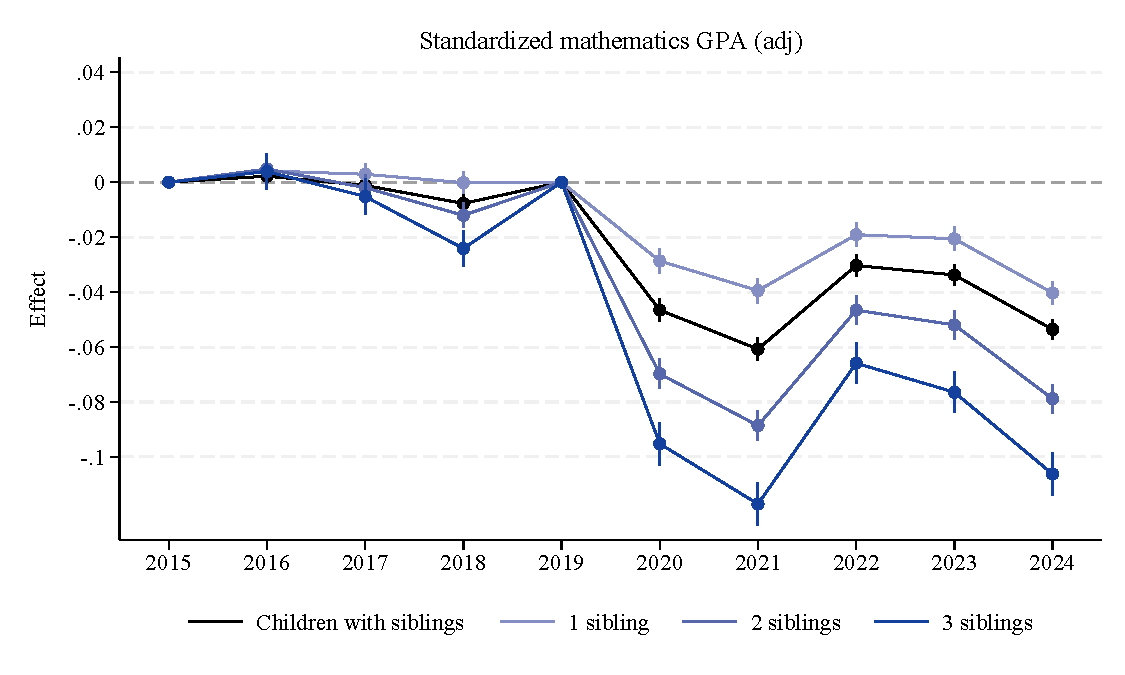
\includegraphics{./FIGURES/Event Study/covid_std_gpa_m_adj_all_all_all_elm_all.pdf}
      }
    }
\end{frame}

\begin{frame}
    \label{update_scott}
    \frametitle{School characteristics}
 {\resizebox{0.9\textwidth}{!}{
       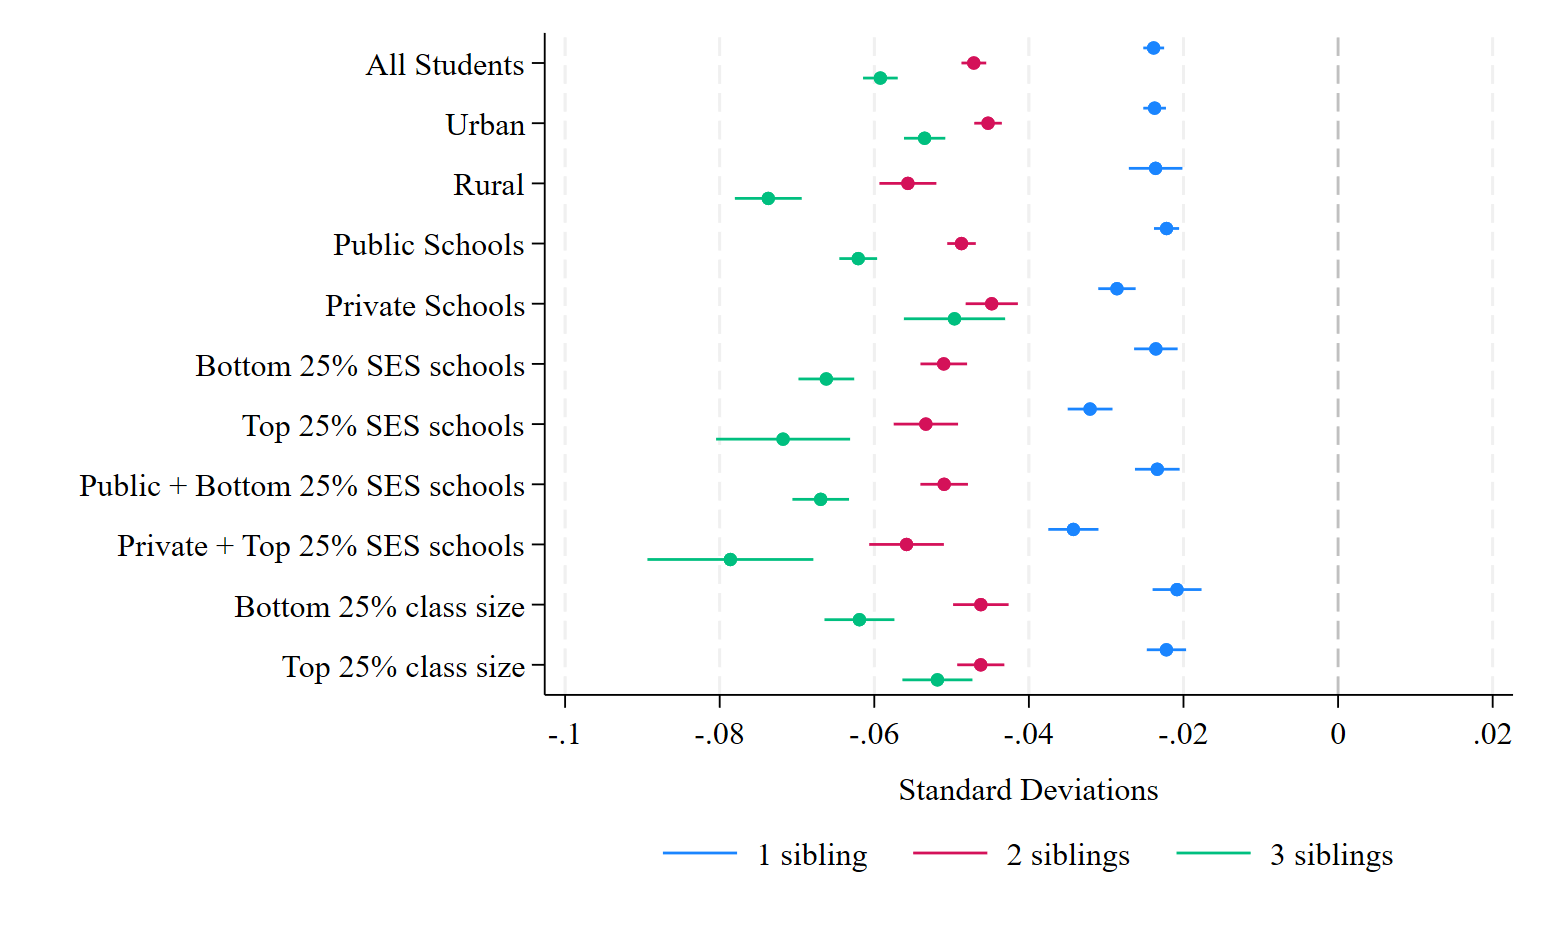
\includegraphics{./FIGURES/TWFE/covid_twfe_A_all_gpa_m_4.png}
      }
    }
\end{frame}

\begin{frame}
    \label{update_scott}
    \frametitle{Student demographics}
 {\resizebox{0.9\textwidth}{!}{
       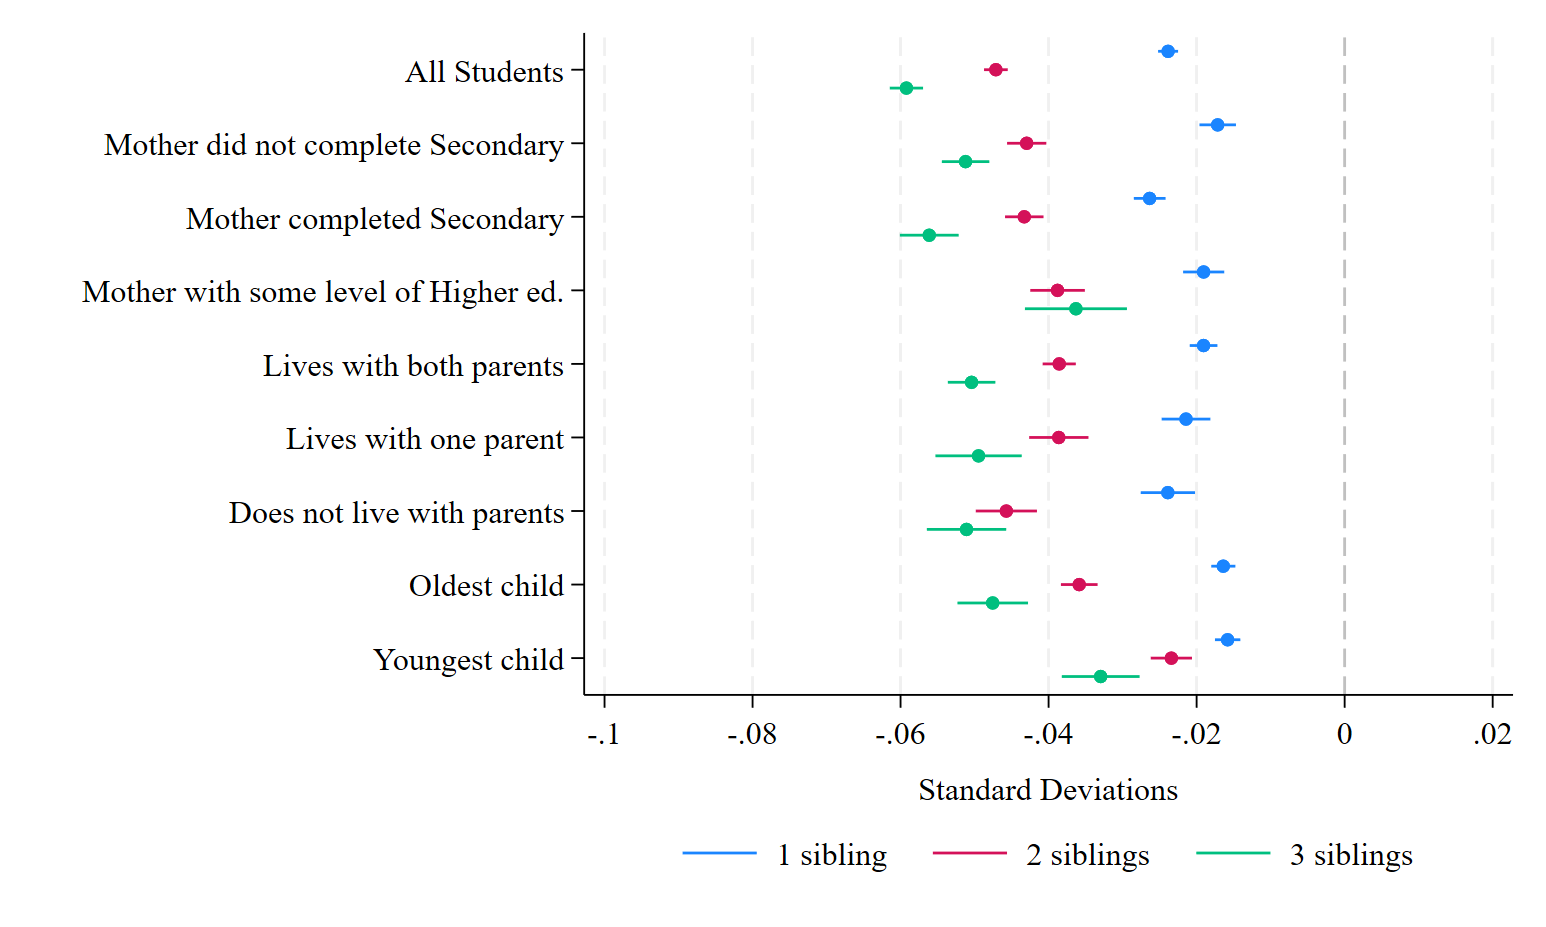
\includegraphics{./FIGURES/TWFE/covid_twfe_B_all_gpa_m_4.png}
      }
    }
\end{frame}

\begin{frame}
    \label{update_scott}
    \frametitle{Family Structure (siblings)}
 {\resizebox{0.9\textwidth}{!}{
       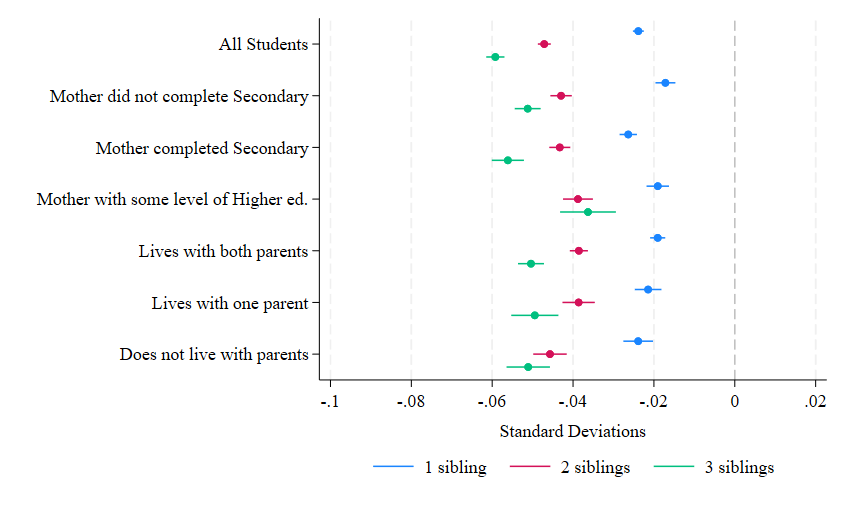
\includegraphics{./FIGURES/TWFE/covid_twfe_C_all_gpa_m_4.png}
      }
    }
\end{frame}

\begin{frame}
    \label{update_scott}
    \frametitle{Family Structure (parents)}
 {\resizebox{0.9\textwidth}{!}{
       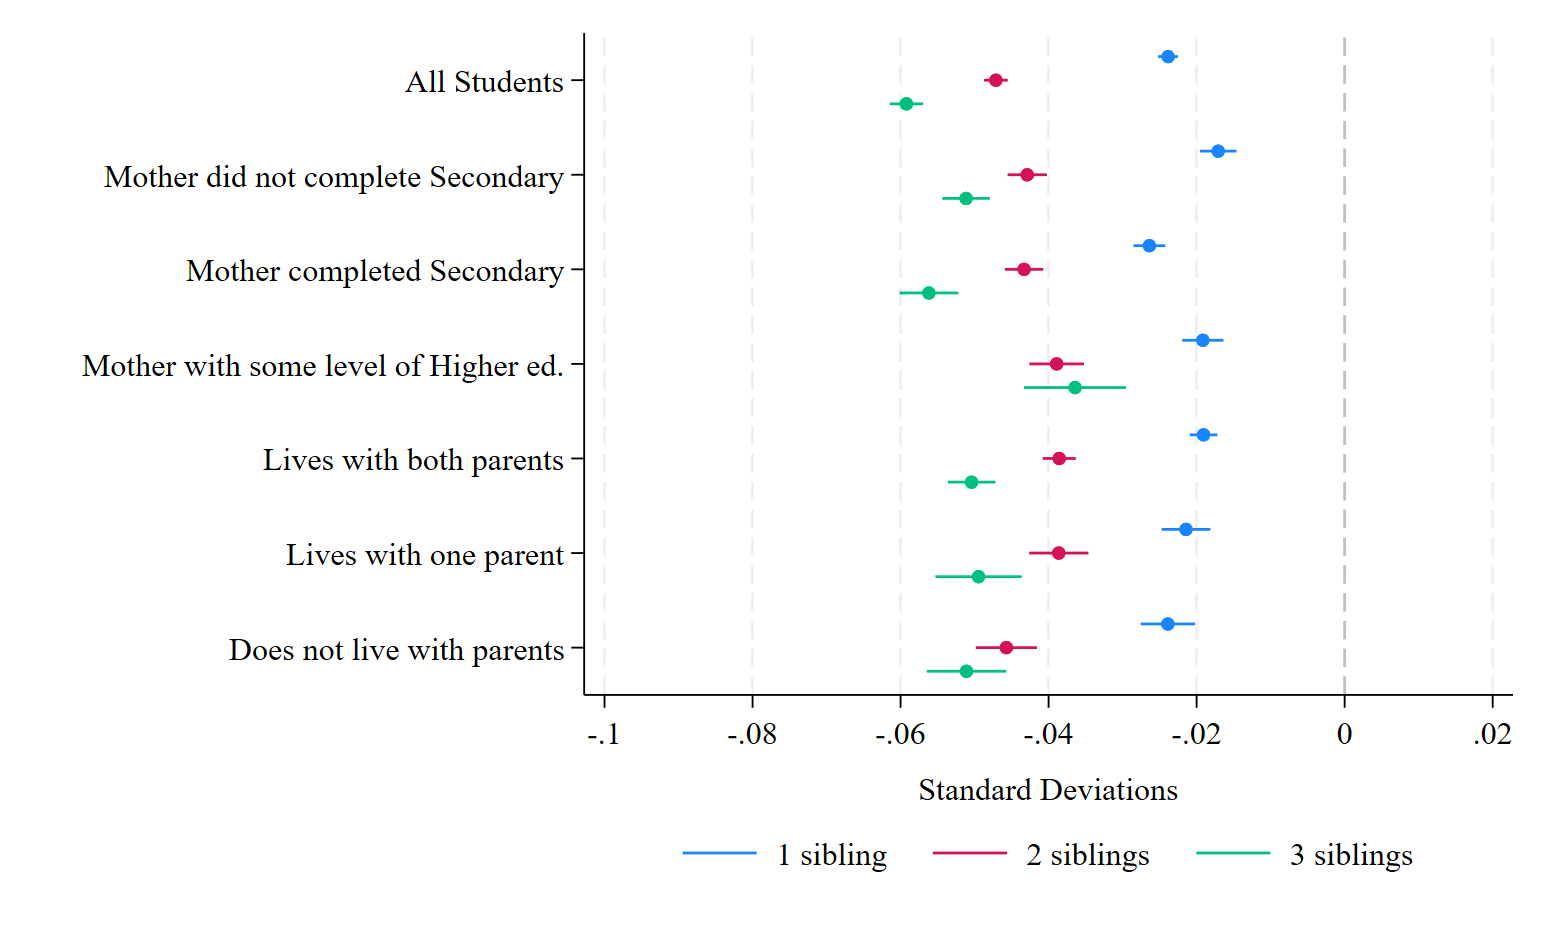
\includegraphics{./FIGURES/TWFE/covid_twfe_D_all_gpa_m_4.png}
      }
    }
\end{frame}

\section{International Evidence - PISA}

\begin{frame}
    \label{update_scott}
    \frametitle{The distribution of gaps moves down}
        {\resizebox{0.9\textwidth}{!}{
       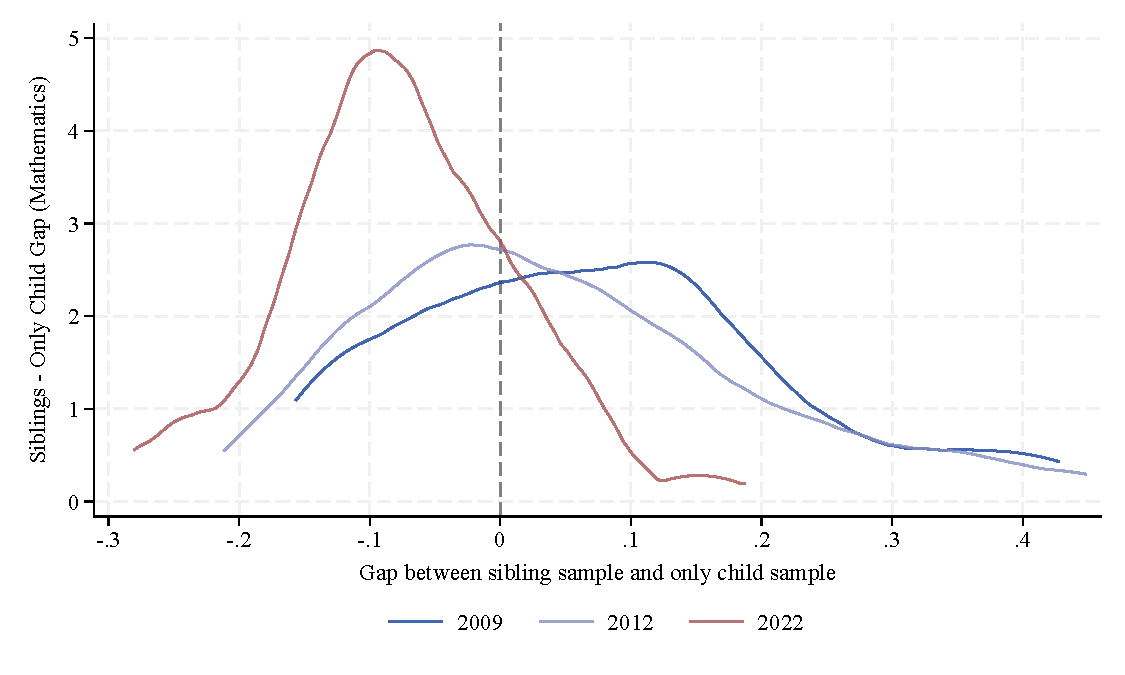
\includegraphics{./FIGURES/Descriptive/PISA_gap_PV1MATH_histogram_2009_2022.pdf}
      }
    }
\end{frame}

\begin{frame}
    \label{update_scott}
    \frametitle{Raw DID vs school closures}
        {\resizebox{0.9\textwidth}{!}{
       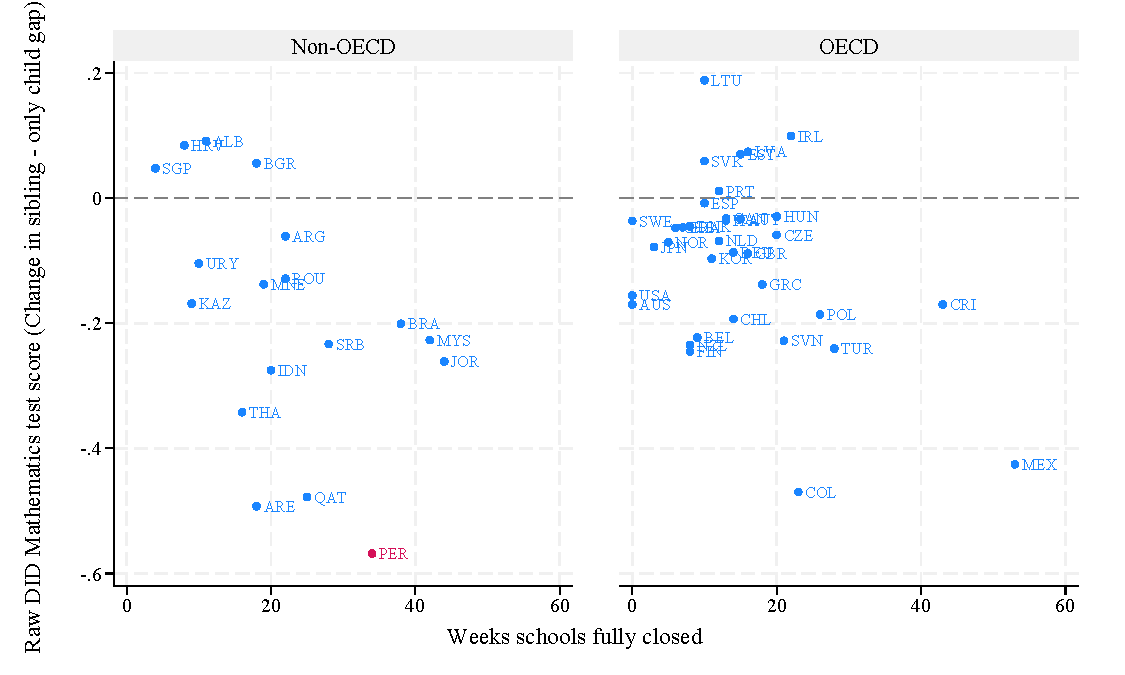
\includegraphics{./FIGURES/Descriptive/PISA_raw_DID_PV1MATH_full.pdf}
      }
    }
\end{frame}

\begin{frame}
    \label{update_scott}
    \frametitle{Raw DID vs school closures}
        {\resizebox{0.9\textwidth}{!}{
       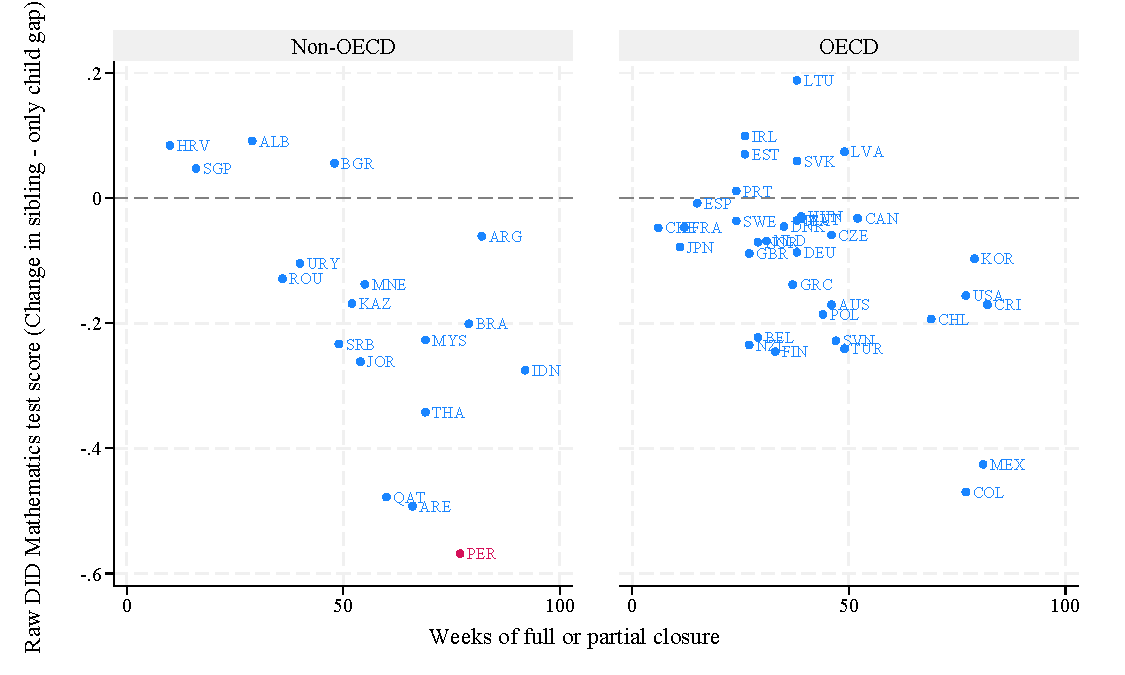
\includegraphics{./FIGURES/Descriptive/PISA_raw_DID_PV1MATH_not_fully_open.pdf}
      }
    }
\end{frame}

\begin{frame}
    \label{update_scott}
    \frametitle{Raw DID vs school closures}
        {\resizebox{0.9\textwidth}{!}{
       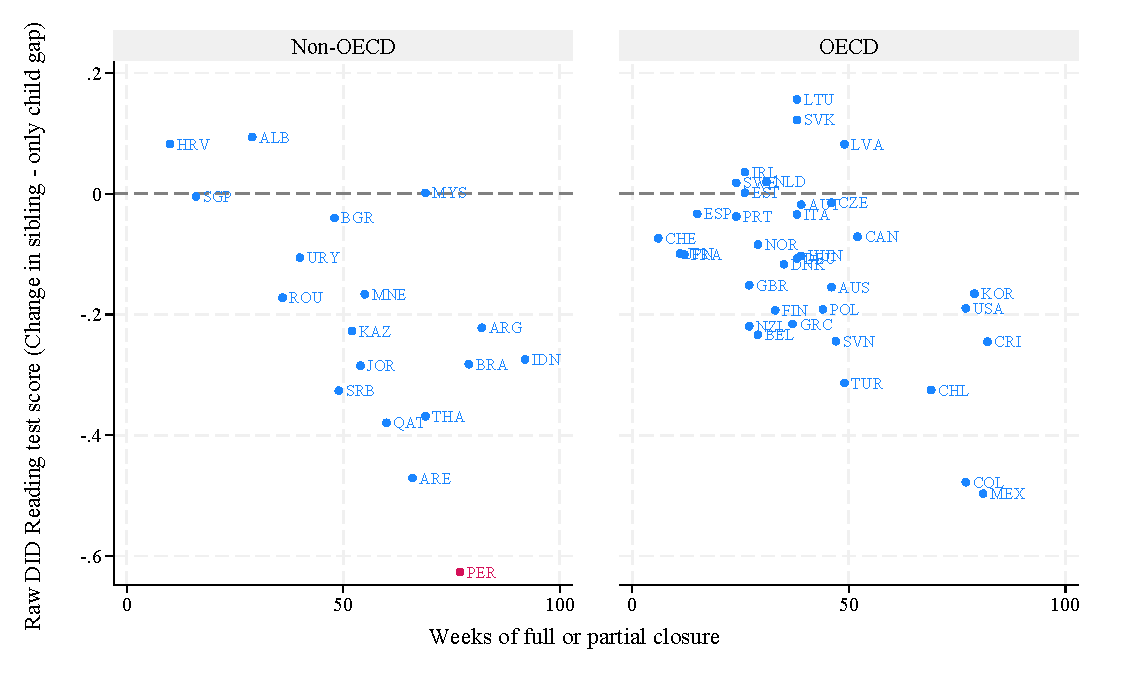
\includegraphics{./FIGURES/Descriptive/PISA_raw_DID_PV1READ_not_fully_open.pdf}
      }
    }
\end{frame}

\section{Change in parental investments}


\begin{frame}
    \frametitle{Parental Investment mechanism}
    \begin{itemize}
        \item Current Hypothesis: During Covid, education relied more on parents than on school
        \item Given limited parent's time, more children means less quality of education
        \item A persistent gap might also be explained by persistent changes in the education production function. 
        \item Did parental input increase during COVID? 
        \item Is it still higher than before COVID?
    \end{itemize}
\end{frame}

\begin{frame}
    \label{update_scott}
    \frametitle{Increase in parental Home-schooling (USA)}
        {\resizebox{0.9\textwidth}{!}{
       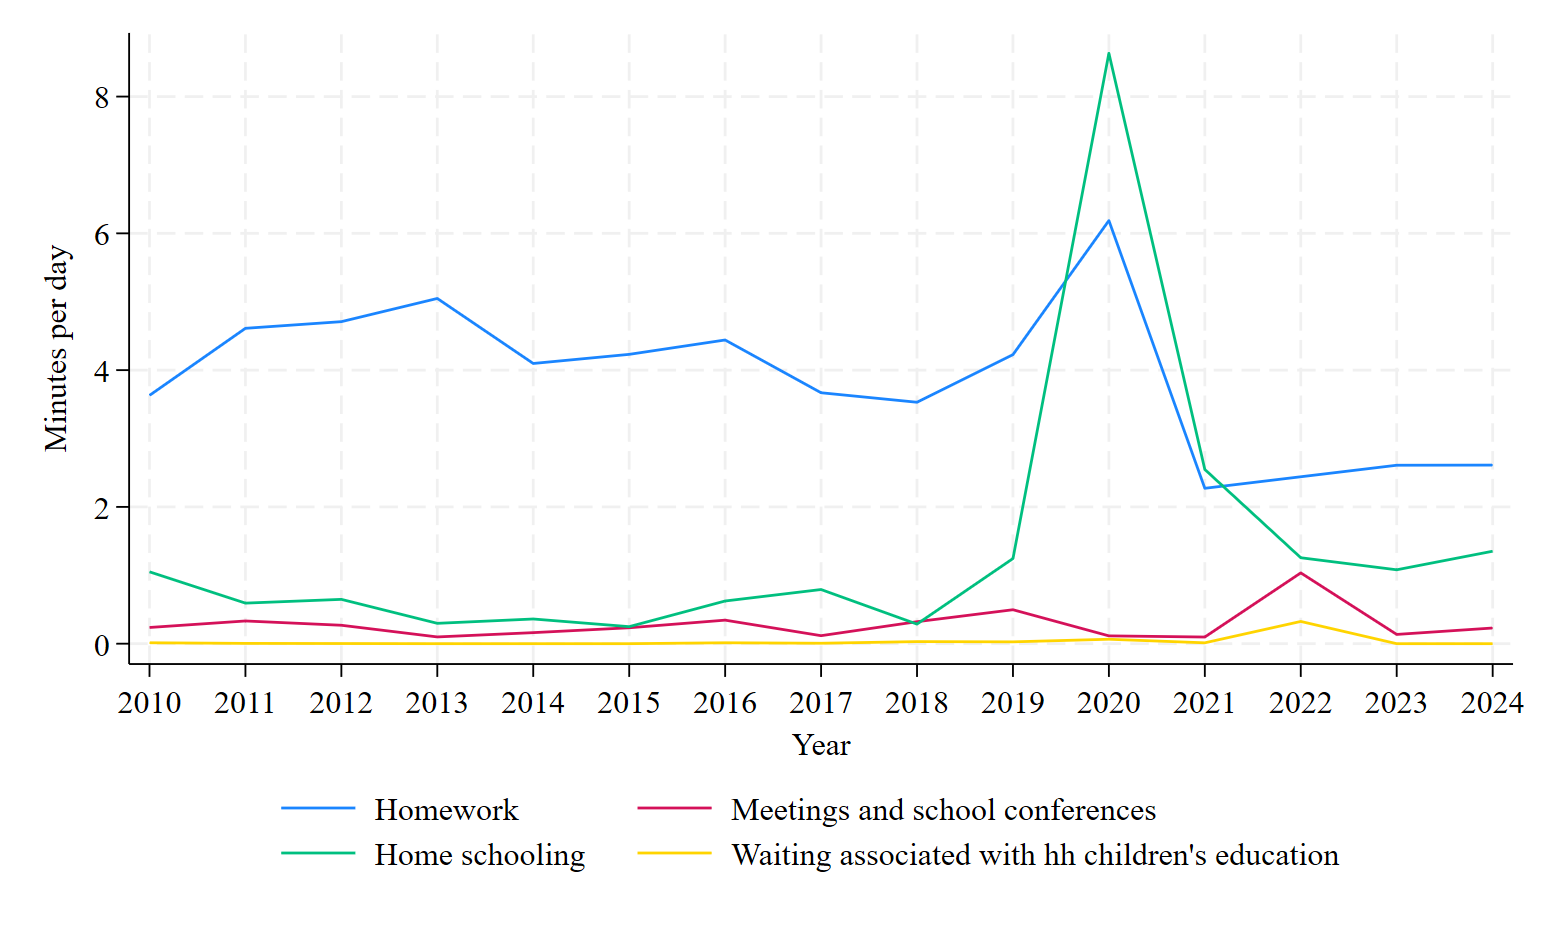
\includegraphics{./FIGURES/Descriptive/ATU_B_0-5.png}
      }
    }
\end{frame}

\begin{frame}
    \label{update_scott}
    \frametitle{Total time spent in care}
        {\resizebox{0.9\textwidth}{!}{
       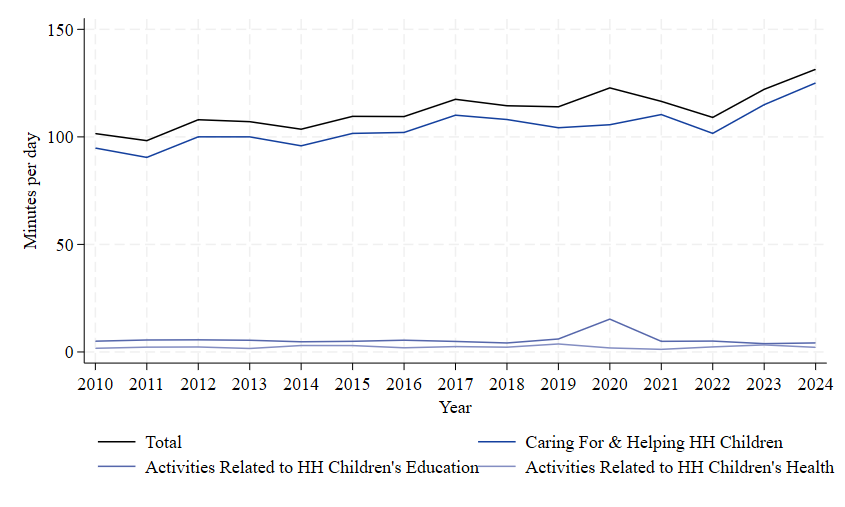
\includegraphics{./FIGURES/Descriptive/ATU_summary_0-5.png}
      }
    }
\end{frame}

\begin{frame}
    \frametitle{Parental Investment vs $\#$ of children}
    \begin{itemize}
        \item Using Peru surveys, I look at the relation between a standardized index of parental investment in education and number of children
        \item Relation becomes more negative after COVID
    \end{itemize}
\end{frame}

\begin{frame}
    \frametitle{Parental investment vs $\#$ of children - 2nd grade}
    \makebox[0.1\width][l]{
\resizebox{\textwidth}{!}{
\begin{tabular}{lcccccc}
\toprule
\cmidrule(lr){2-7}
& \multicolumn{2}{c}{2015} & \multicolumn{2}{c}{2022} & \multicolumn{2}{c}{2023} \\
\cmidrule(lr){2-3} \cmidrule(lr){4-5} \cmidrule(lr){6-7}  
& (1) & (2) & (3) & (4) & (5) & (6) \\
\bottomrule
&  &  &  &  & & \\
2 Children          &       0.010   &       0.015** &      -0.078***&      -0.077***&      -0.096***&      -0.067***\\
                    &     (0.006)   &     (0.006)   &     (0.007)   &     (0.007)   &     (0.024)   &     (0.023)   \\
3 Children          &      -0.113***&      -0.055***&      -0.259***&      -0.190***&      -0.311***&      -0.201***\\
                    &     (0.008)   &     (0.007)   &     (0.008)   &     (0.008)   &     (0.031)   &     (0.031)   \\
4 Children          &      -0.253***&      -0.129***&      -0.416***&      -0.246***&      -0.444***&      -0.240***\\
                    &     (0.010)   &     (0.010)   &     (0.012)   &     (0.013)   &     (0.048)   &     (0.048)   \\
Controls            &          No   &         Yes   &          No   &         Yes   &          No   &         Yes   \\
                    &               &               &               &               &               &               \\
Observations        &     133,361   &     133,349   &     116,232   &      96,094   &       8,934   &       7,738   \\
 

\bottomrule
\end{tabular}
}
}

\end{frame}

\begin{frame}
    \frametitle{Parental investment vs $\#$  of children - 8th grade}
    \makebox[0.1\width][l]{
\resizebox{\textwidth}{!}{
\begin{tabular}{lcccc}
\toprule
\cmidrule(lr){2-5}
& \multicolumn{2}{c}{2015} & \multicolumn{2}{c}{2023}  \\
\cmidrule(lr){2-3} \cmidrule(lr){4-5}   
& (1) & (2) & (3) & (4)\\
\bottomrule
&  &  &  &  \\
2 Children          &       0.017***&       0.028***&      -0.003   &      -0.002   \\
                    &     (0.004)   &     (0.004)   &     (0.007)   &     (0.007)   \\
3 Children          &      -0.011***&       0.023***&      -0.068***&      -0.052***\\
                    &     (0.004)   &     (0.004)   &     (0.008)   &     (0.008)   \\
4 Children          &      -0.029***&       0.032***&      -0.107***&      -0.064***\\
                    &     (0.006)   &     (0.006)   &     (0.011)   &     (0.012)   \\
Controls            &          No   &         Yes   &          No   &         Yes   \\
                    &               &               &               &               \\
Observations        &     426,938   &     426,673   &     113,562   &     112,143   \\
 

\bottomrule
\end{tabular}
}
}

\end{frame}







\section{School entry cutoff as exogeneity}

\begin{frame}
    \label{update_scott}
    \frametitle{Exposure to school closures}
    \begin{itemize}
        \item There are clear school-age entry cutoffs
        \item Pre-covid, having a child start school will mean less childcare responsibilities $\rightarrow$ more time for older child
        \item Post-covid, having a child start school will mean more education responsibilities $\rightarrow$ less time for older child
        %\item There is an age-entry cutoff in schools. Some kids are delayed and others have to enroll in 1st grade.
        %\item Can this be a source of variation? Not only of the effects of the pandemic but also as source of variation in 'siblings in school' that may require extra parental attention.
        %but a DID of family size and exposure to pandemic?
        %\item $\approx$ 1500 students per day
        %\item I know how Covid was dealt with for elementary (1-6), but not sure what K and below meant. Some students are in the data 3 years before elementary. Was there services during COVID?
    \end{itemize}
\end{frame}

\begin{frame}
    \label{update_scott}
    \frametitle{Potential variations}
    \begin{itemize}
        \item PreK-K starting age
        \item \textbf{1st grade starting age}
        \item graduating from primary
        \item graduating from school
        %\item Exposure to the pandemic and future outcomes
        %\item Having a younger sibling start school during pandemic. (randomness over +1 sibling in school).
        %\item Exposure to covid while having siblings or not (Is this the same as my diff in diff?). The randomness is in being exposed to pandemic or not, not in having a sibling.
    \end{itemize}
\end{frame}

\begin{frame}
    \label{update_scott}
    \frametitle{School age entry cutoffs}
 {\resizebox{0.9\textwidth}{!}{
       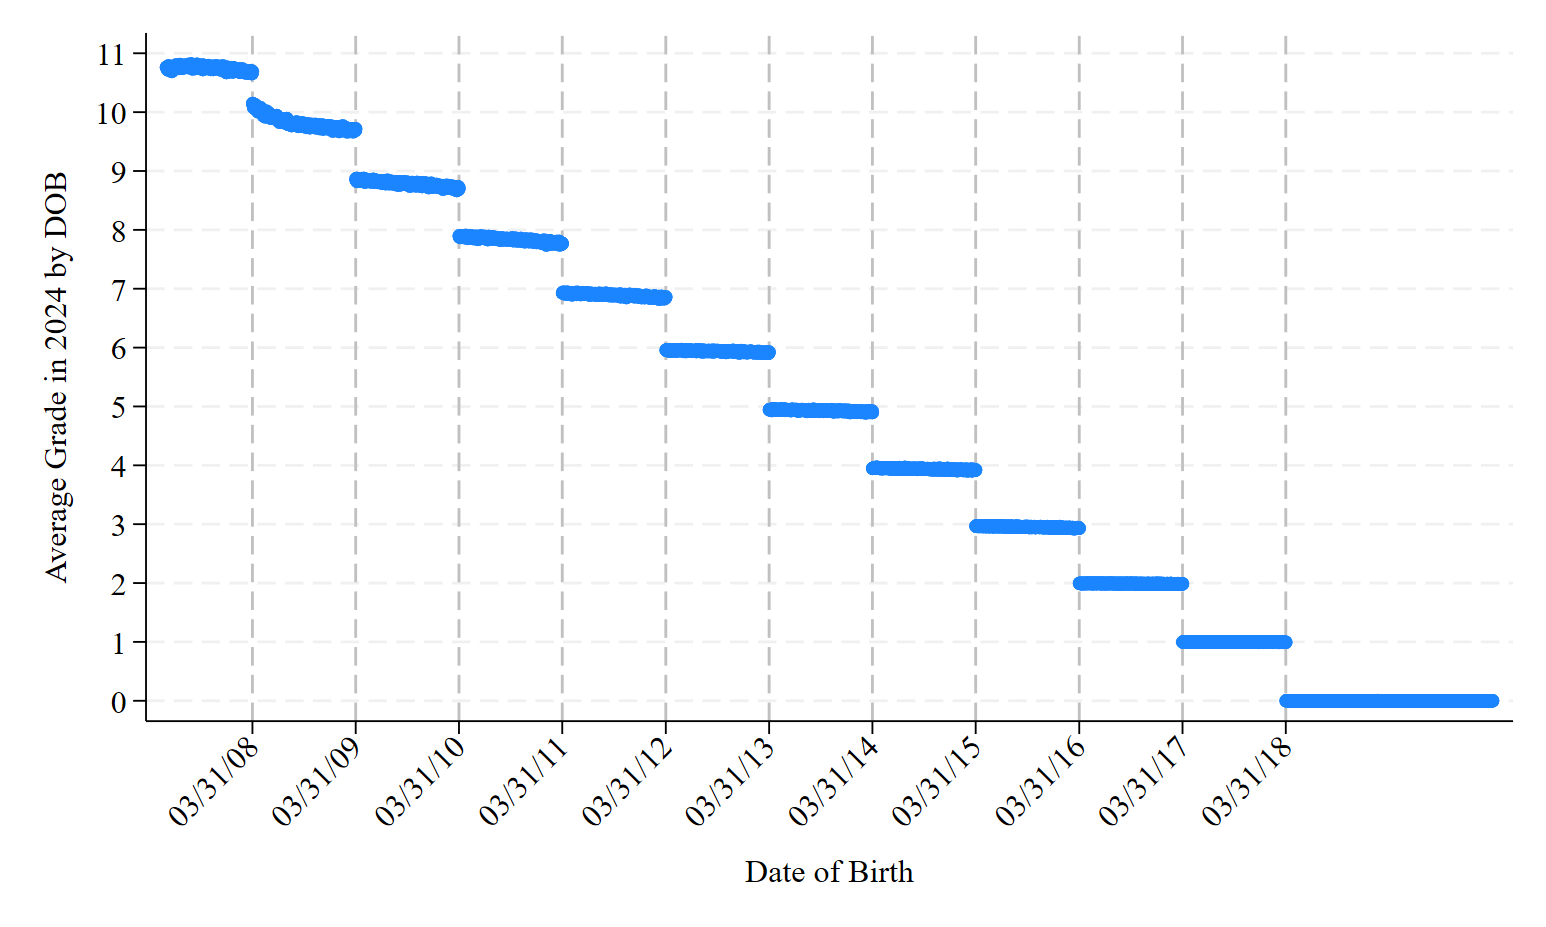
\includegraphics{./FIGURES/Descriptive/dob_cutoffs.png}
      }
    }
\end{frame}

\begin{frame}
    \label{update_scott}
    \frametitle{A delay in school start pre-covid means more childcare}
 {\resizebox{0.9\textwidth}{!}{
       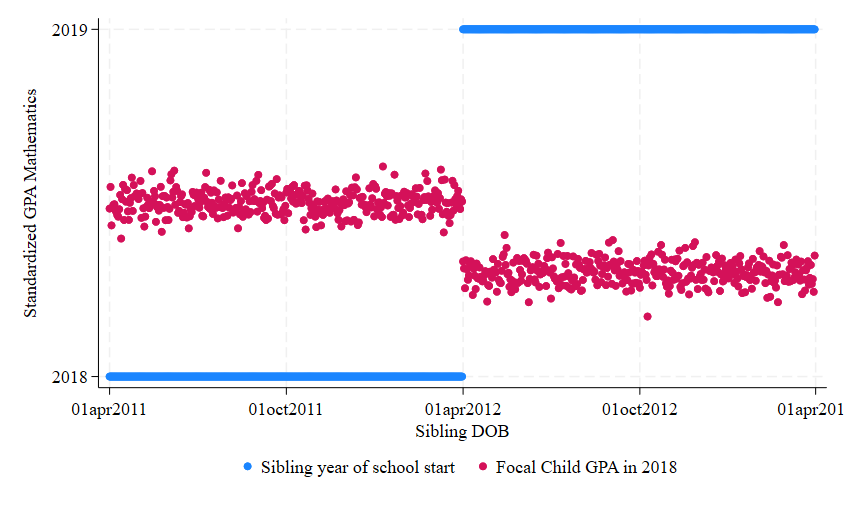
\includegraphics{./FIGURES/Descriptive/example_pre_covid.png}
      }
    }
\end{frame}



\begin{frame}
    \label{update_scott}
    \frametitle{A delay in school start post-covid means less education responsibility}
 {\resizebox{0.9\textwidth}{!}{
       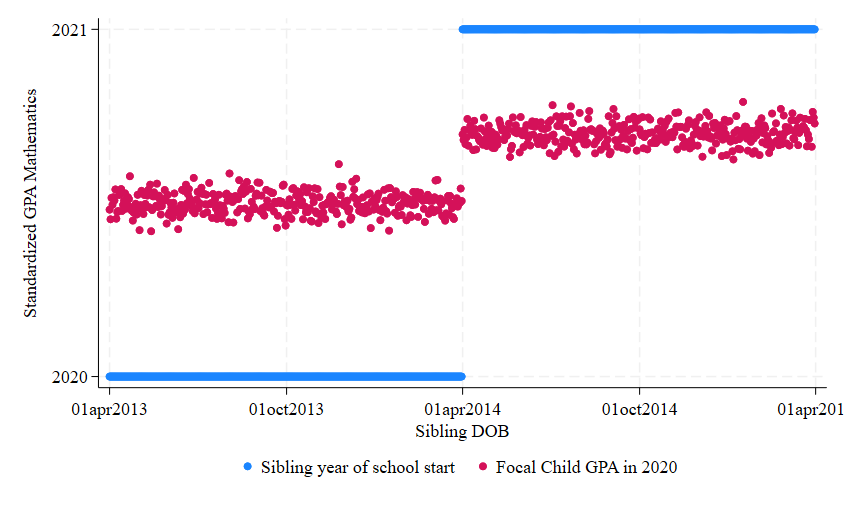
\includegraphics{./FIGURES/Descriptive/example_post_covid.png}
      }
    }
\end{frame}


\begin{frame}
    \frametitle{RD results for HH = 2 children}
    \makebox[0.1\width][l]{
\resizebox{\textwidth}{!}{
\begin{tabular}{lcccc}
\toprule
\cmidrule(lr){2-5}
& 2018 & 2019 & 2020 & 2021 \\
& (1) & (2) & (3) & (4)  \\
\bottomrule
&  &  &  & \\
ABOVE       &      -0.007   &      -0.035** &      -0.012   &      -0.008   \\
            &     (0.012)   &     (0.012)   &     (0.012)   &     (0.011)   \\
            &               &               &               &               \\
Observations&     105,723   &     117,154   &     106,496   &     115,217   \\

\bottomrule
\end{tabular}
}
}

\end{frame}

\begin{frame}
    \frametitle{RD results for HH = 3 children (oldest-middle}
    \makebox[0.1\width][l]{
\resizebox{\textwidth}{!}{
\begin{tabular}{lcccc}
\toprule
\cmidrule(lr){2-5}
& 2018 & 2019 & 2020 & 2021 \\
& (1) & (2) & (3) & (4)  \\
\bottomrule
&  &  &  & \\
ABOVE       &      -0.019   &      -0.038** &      -0.005   &      -0.030   \\
            &     (0.016)   &     (0.016)   &     (0.020)   &     (0.021)   \\
            &               &               &               &               \\
Observations&      59,335   &      54,530   &      37,477   &      33,225   \\

\bottomrule
\end{tabular}
}
}

\end{frame}


\begin{frame}
    \frametitle{RD results for HH = 3 children (middle-youngest}
    \makebox[0.1\width][l]{
\resizebox{\textwidth}{!}{
\begin{tabular}{lcccc}
\toprule
\cmidrule(lr){2-5}
& 2018 & 2019 & 2020 & 2021 \\
& (1) & (2) & (3) & (4)  \\
\bottomrule
&  &  &  & \\
ABOVE       &      -0.023   &      -0.031*  &       0.033*  &       0.001   \\
            &     (0.018)   &     (0.016)   &     (0.017)   &     (0.017)   \\
            &               &               &               &               \\
Observations&      48,913   &      56,358   &      48,994   &      53,038   \\

\bottomrule
\end{tabular}
}
}

\end{frame}



\section{Other TWFE: Age gap, same sex, middle child, school size}

\begin{frame}
    \label{update_scott}
    \frametitle{Thinking about the literature/models}
    \begin{itemize}
        \item If parents are replacing teachers, we could expect a bigger role where teachers had a bigger share (small class size, teacher/student ration)
        \item Middle child is more affected than older/younger
        \item Age gap and fight for resources
    \end{itemize}
\end{frame}


\begin{frame}
    \label{update_scott}
    \frametitle{TWFE}
 {\resizebox{0.9\textwidth}{!}{
       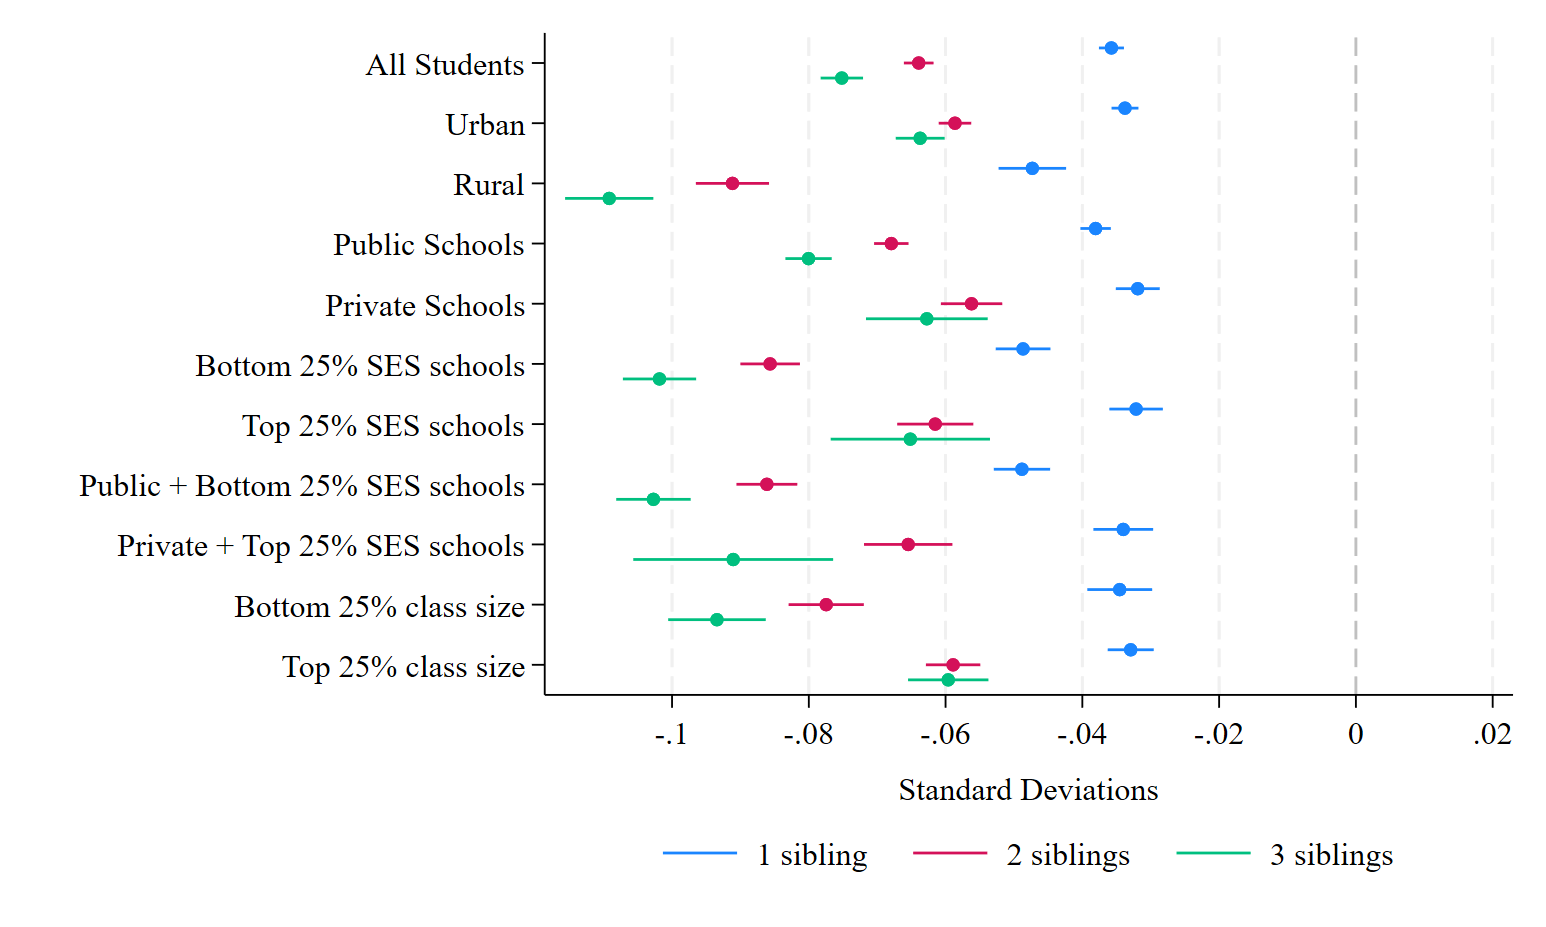
\includegraphics{./FIGURES/TWFE/covid_twfe_A_elm_gpa_c_adj_4.png}
      }
    }
\end{frame}

\begin{frame}
    \label{update_scott}
    \frametitle{TWFE}
 {\resizebox{0.9\textwidth}{!}{
       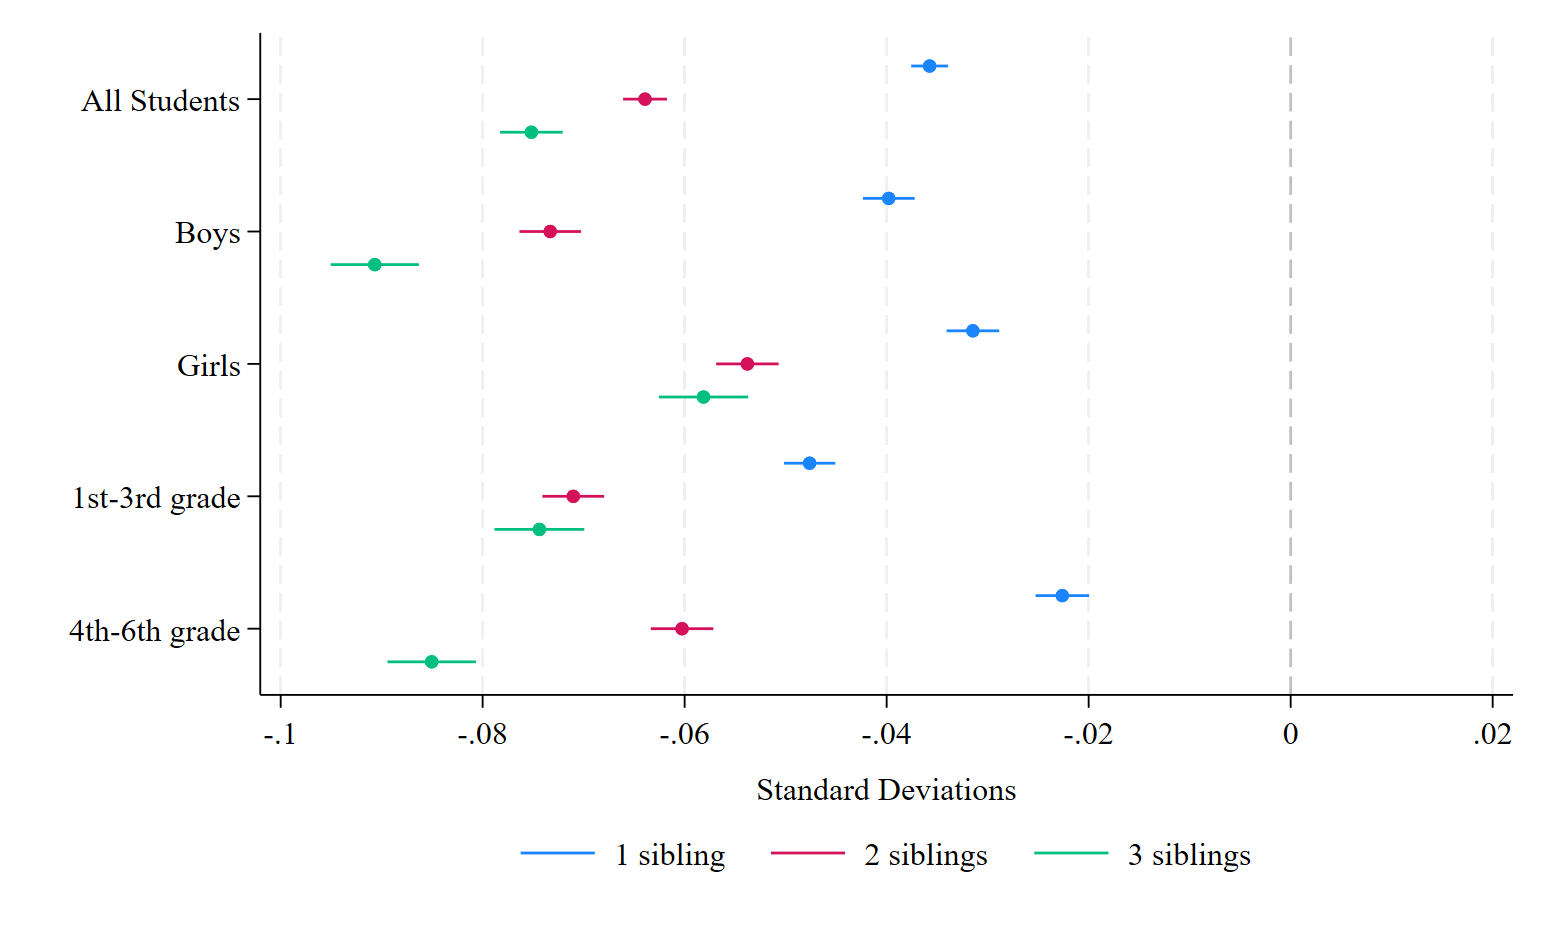
\includegraphics{./FIGURES/TWFE/covid_twfe_B_elm_gpa_c_adj_4.png}
      }
    }
\end{frame}

\begin{frame}
    \label{update_scott}
    \frametitle{TWFE}
 {\resizebox{0.9\textwidth}{!}{
       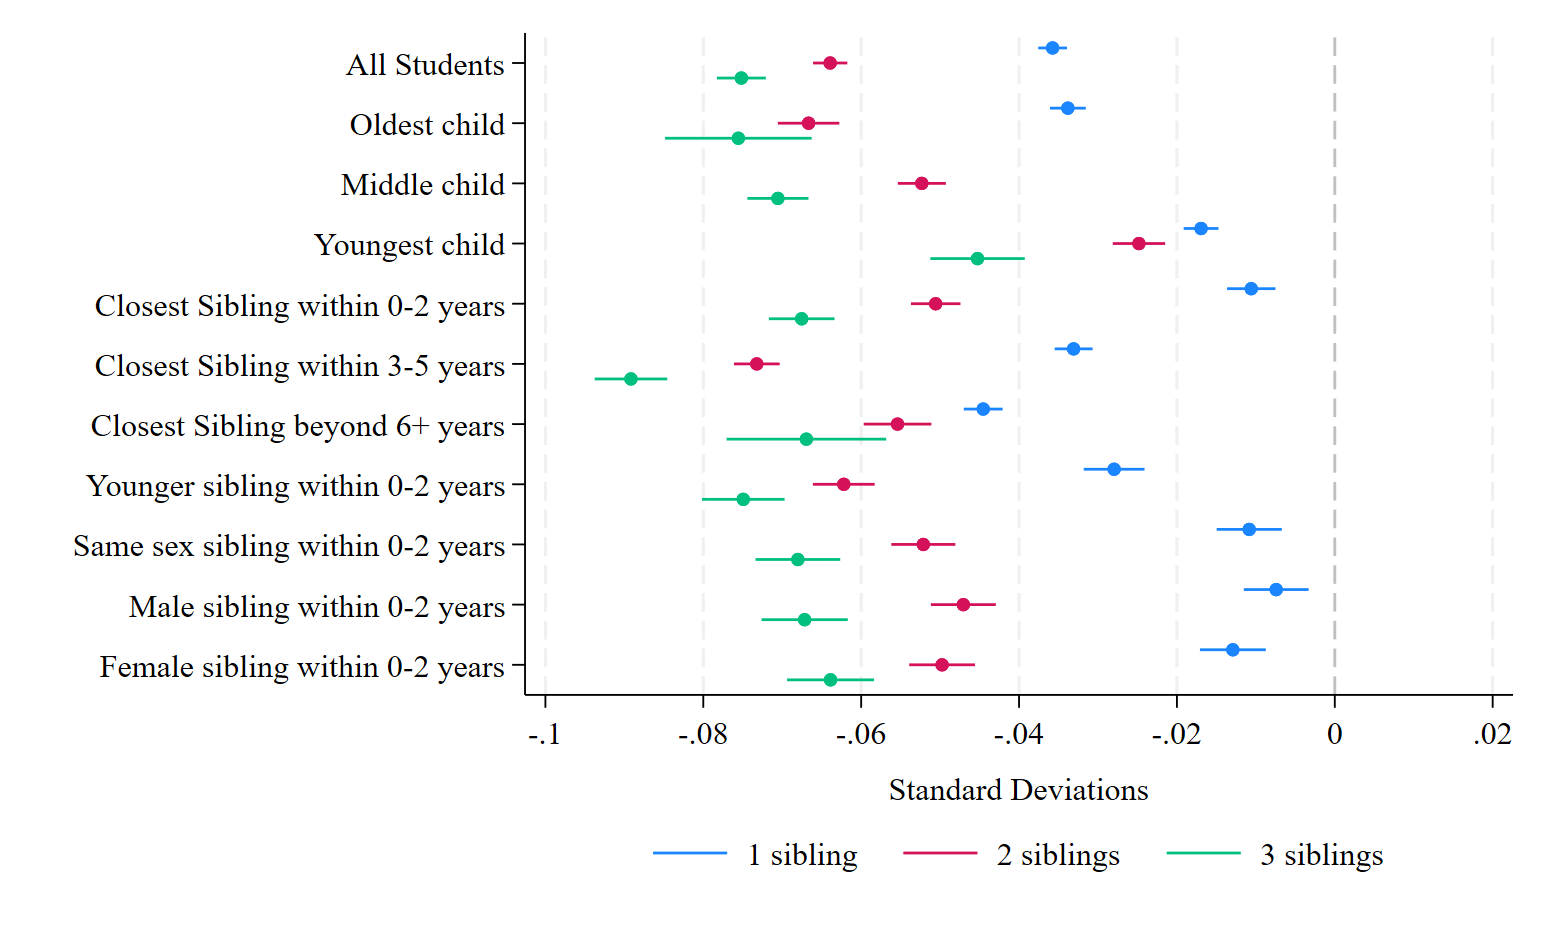
\includegraphics{./FIGURES/TWFE/covid_twfe_C_elm_gpa_c_adj_4.png}
      }
    }
\end{frame}

\begin{frame}
    \label{update_scott}
    \frametitle{TWFE}
 {\resizebox{0.9\textwidth}{!}{
       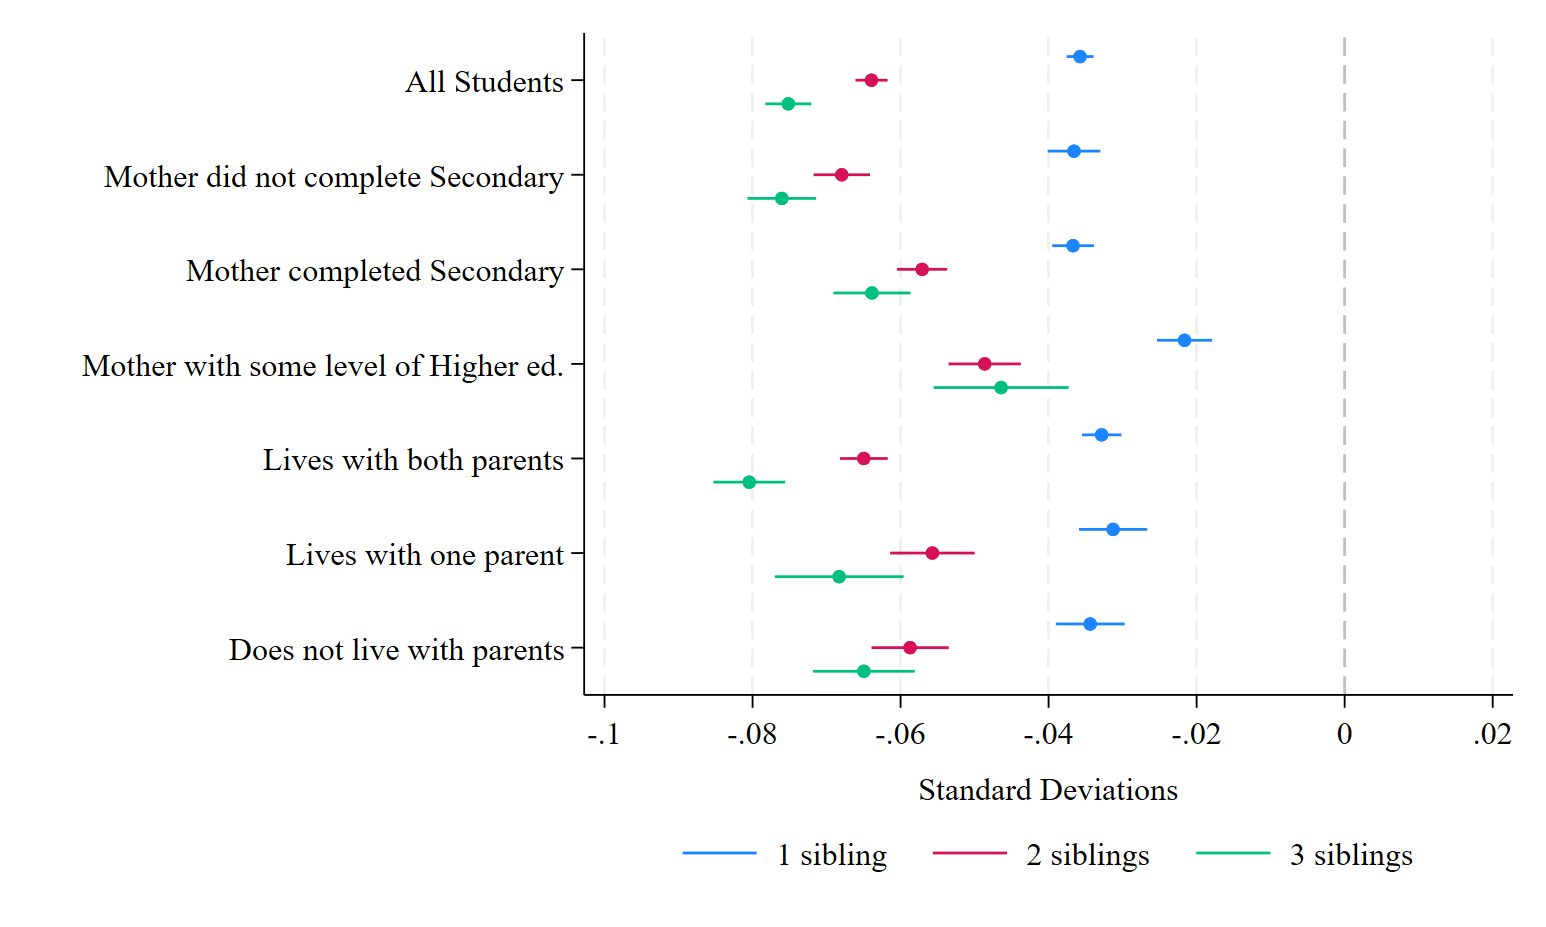
\includegraphics{./FIGURES/TWFE/covid_twfe_D_elm_gpa_c_adj_4.png}
      }
    }
\end{frame}



\section{Next Steps}

\begin{frame}
    \label{update_scott}
    \frametitle{Next Steps}
    \begin{itemize}
        \item Other cutoffs? Primary and HS graduation cutoffs.
        \item Having a sibling born during COVID vs non-COVID?
    \end{itemize}
\end{frame}

\section{Job Market}

\begin{frame}
    \label{update_scott}
    \frametitle{Job Talk}
    \begin{enumerate}
        \item 8/29 (internal DLP); 9/15 (department-wide)
        \item 9/12 (internal DLP); 9/29 (department-wide)
        \item 9/19 (internal DLP); 10/6 (department-wide)
        \item 9/26 (internal DLP); 10/13 (department-wide)
    \end{enumerate}
\end{frame}


\begin{frame}
    \label{update_scott}
    \frametitle{Job Market Paper}
    \begin{enumerate}
        \item Thoughts on pursuing this or focusing on my previous research on sibling spillovers?
    \end{enumerate}
\end{frame}

\section{Thanks!}






\section{Grade change criteria}

\begin{frame}
    \label{update_scott}
    \frametitle{Grade distributions pre-covid: Elementary}
 {\resizebox{0.9\textwidth}{!}{
       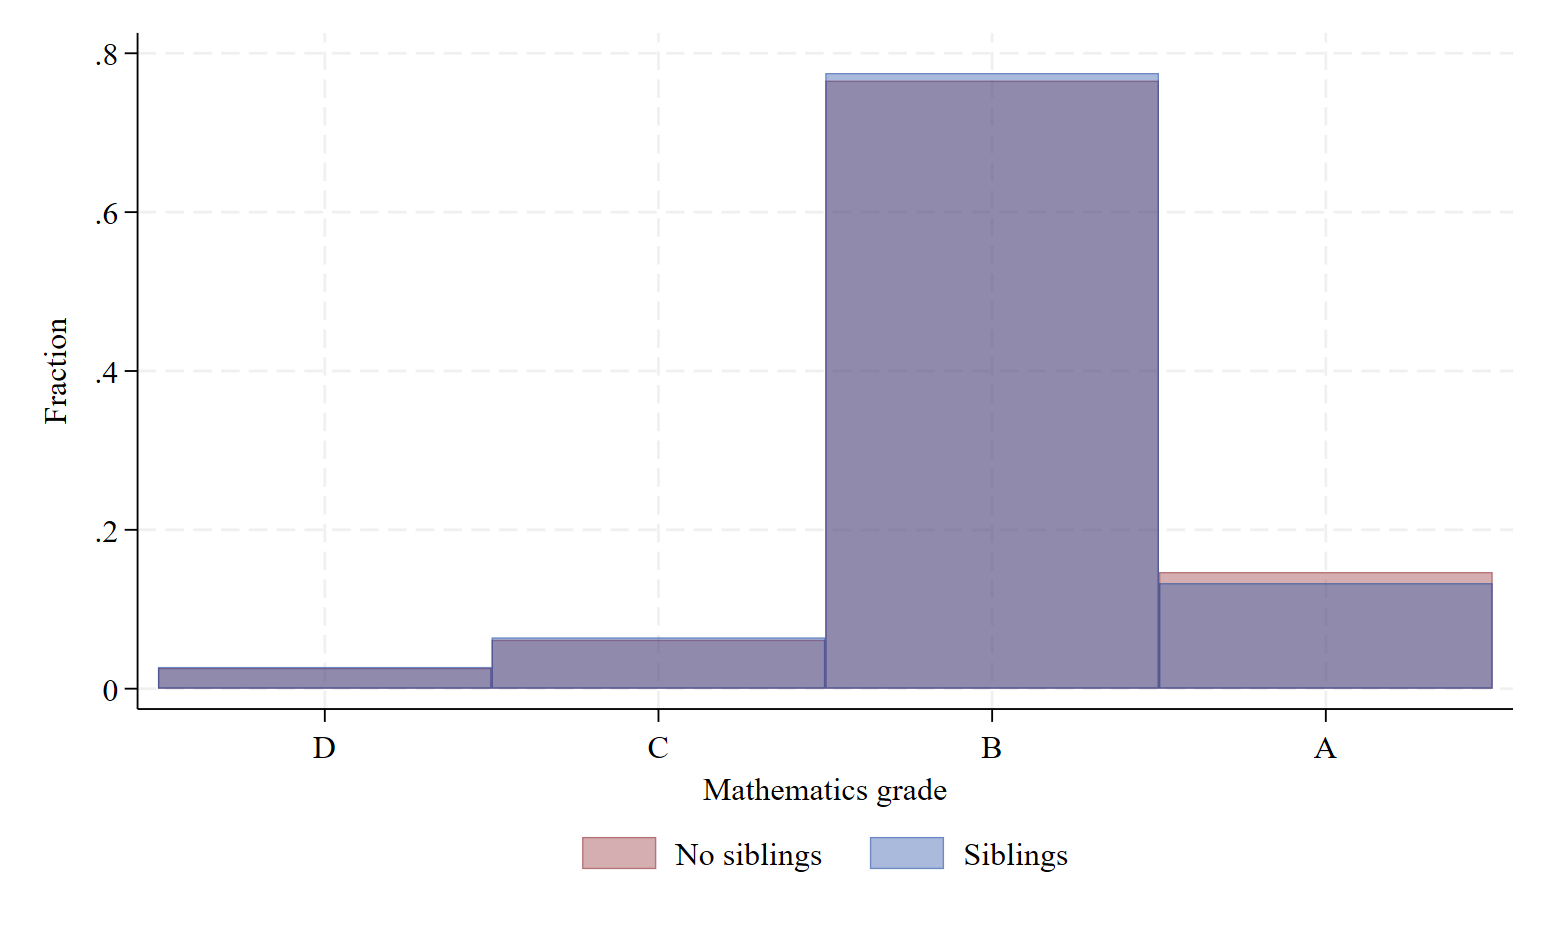
\includegraphics{./FIGURES/Descriptive/histogram_pre_elm.png}
      }
    }
\end{frame}

\begin{frame}
    \label{update_scott}
    \frametitle{Grade distributions pre-covid: Secondary}
 {\resizebox{0.9\textwidth}{!}{
       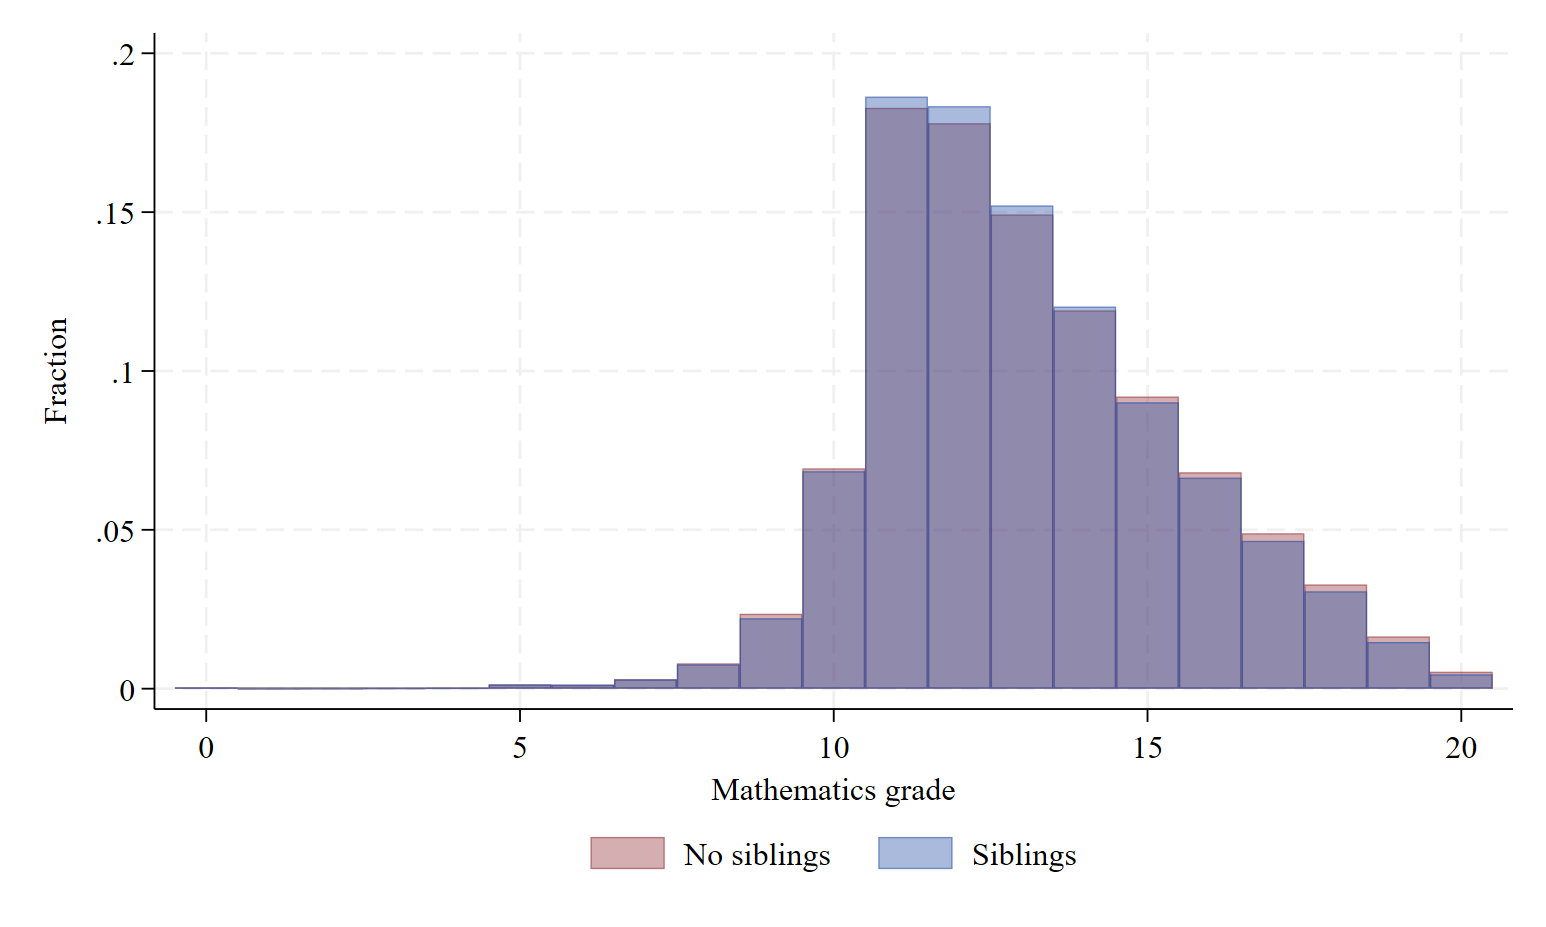
\includegraphics{./FIGURES/Descriptive/histogram_pre_9-10.png}
      }
    }
\end{frame}


\begin{frame}
    \label{update_scott}
    \frametitle{Event Study - Mathematics GPA}
        {\resizebox{0.9\textwidth}{!}{
       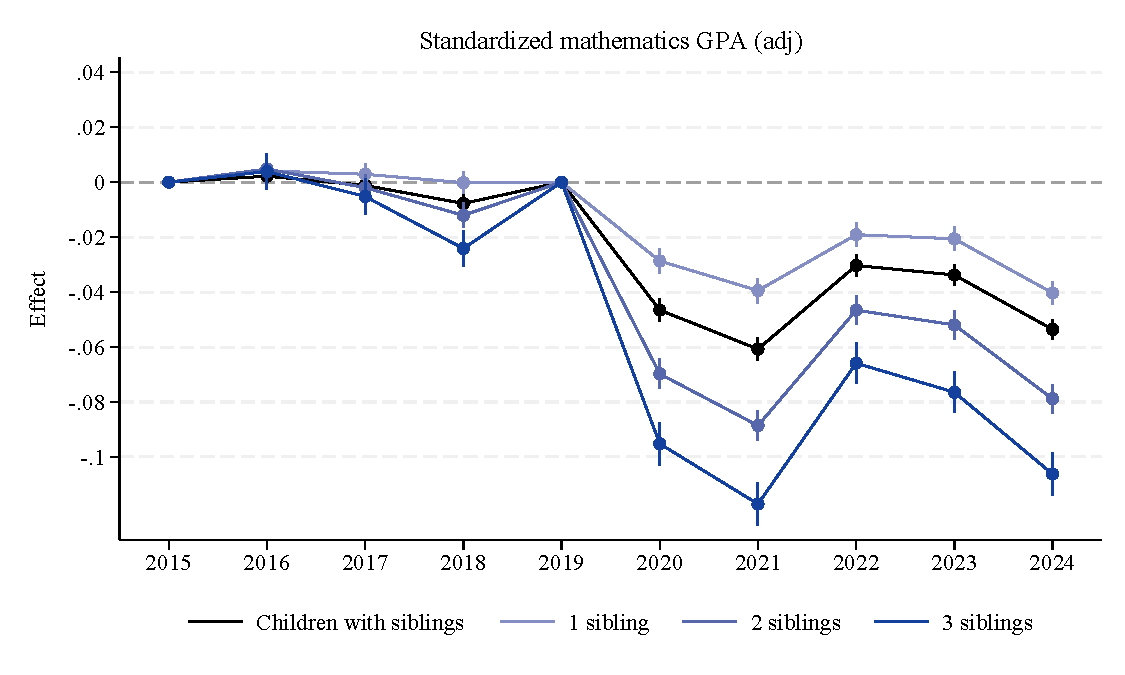
\includegraphics{./FIGURES/Event Study/covid_std_gpa_m_adj_all_all_all_elm_all.pdf}
      }
    }
\end{frame}





\section{Parallel Trends}

\begin{frame}
    \label{update_scott}
    \frametitle{\% of A's in Mathematics}
        {\resizebox{0.9\textwidth}{!}{
       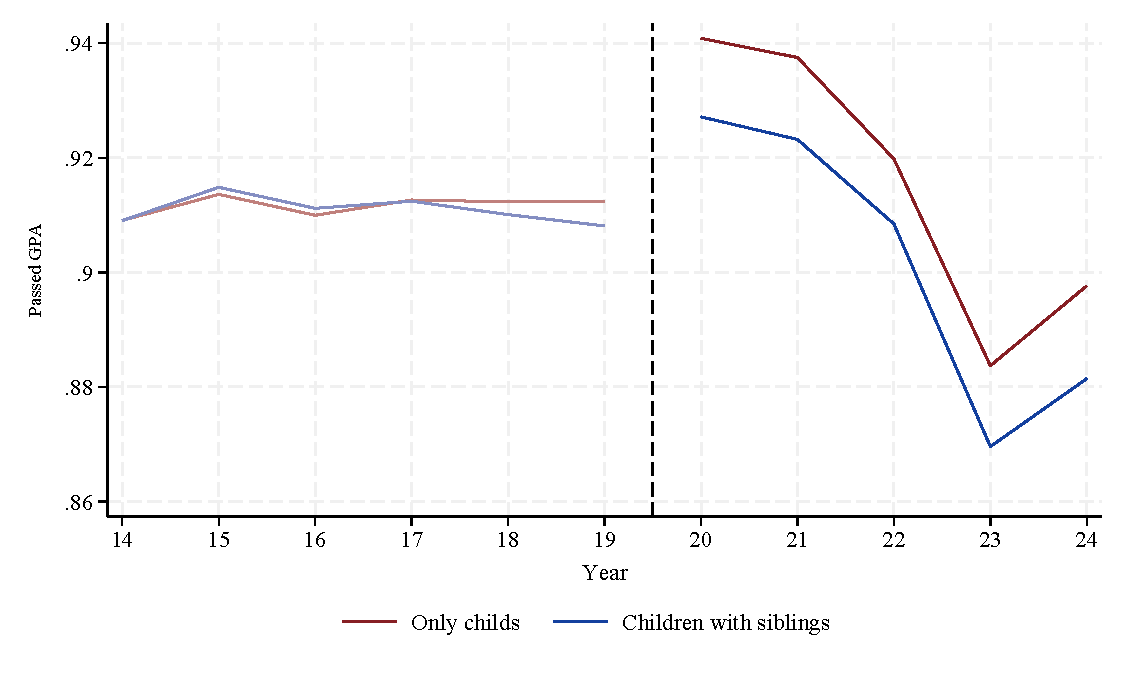
\includegraphics{./FIGURES/Descriptive/raw_total_elm_pass_math.pdf}
      }
    }
\end{frame}

\begin{frame}
    \label{update_scott}
    \frametitle{Standardized GPA in Mathematics}
        {\resizebox{0.9\textwidth}{!}{
       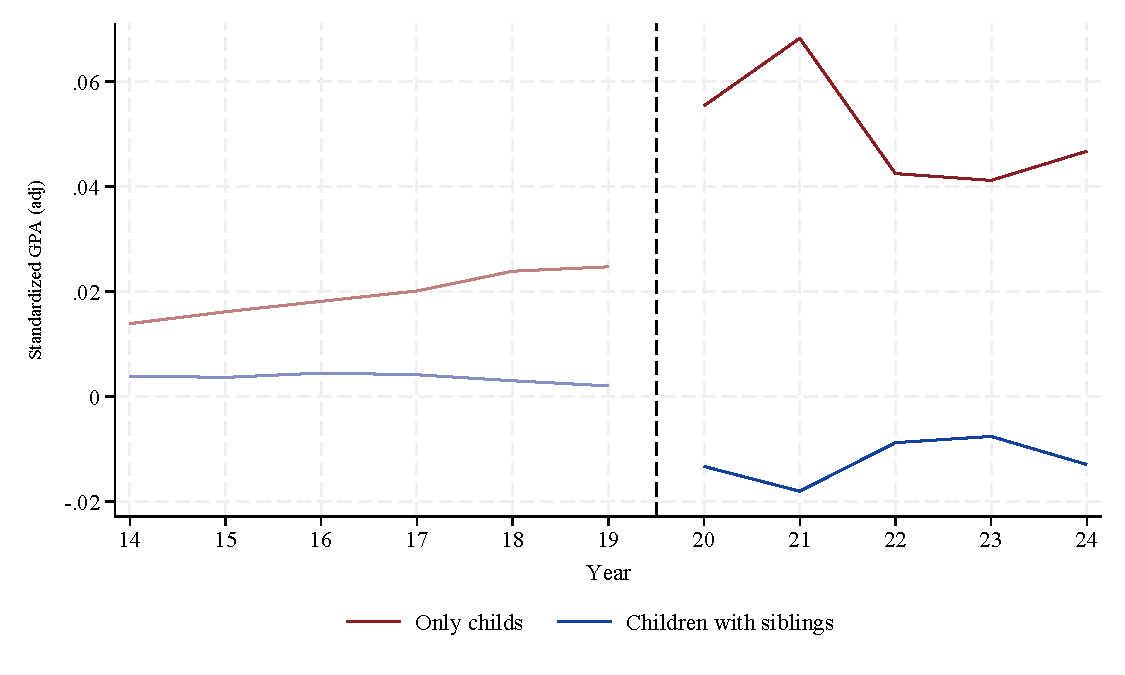
\includegraphics{./FIGURES/Descriptive/raw_total_elm_std_gpa_m_adj.pdf}
      }
    }
\end{frame}

\begin{frame}
    \label{update_scott}
    \frametitle{Standardized GPA in Mathematics}
        {\resizebox{0.9\textwidth}{!}{
       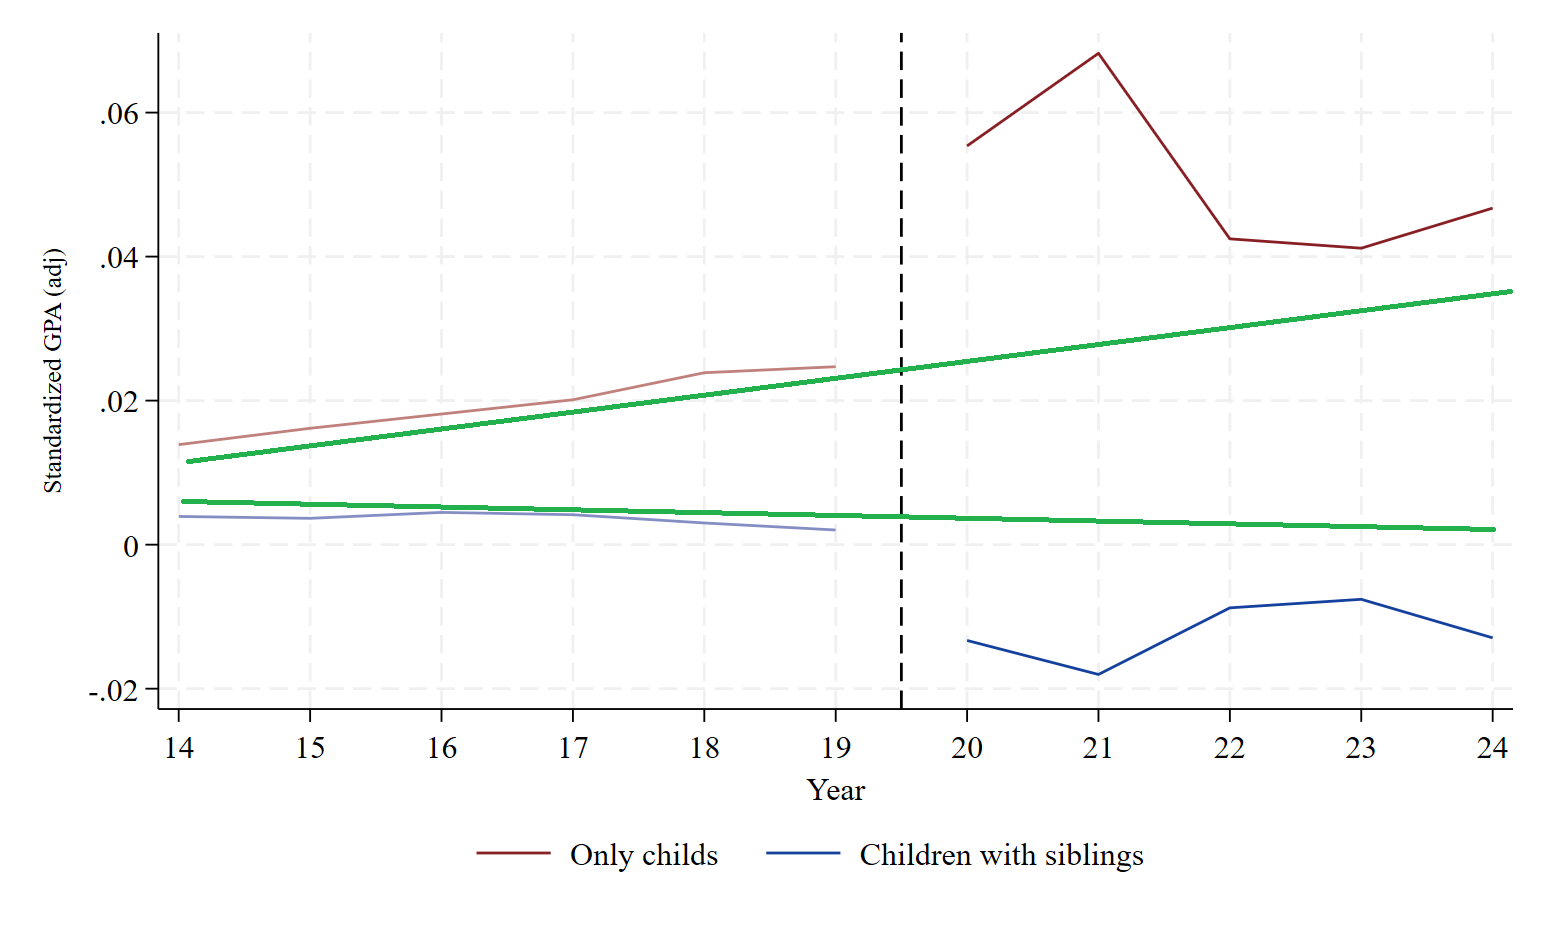
\includegraphics{./FIGURES/Descriptive/parallel_trends.png}
      }
    }
\end{frame}


\section{Thinking about the model}
\begin{frame}
    \label{update_scott}
    \frametitle{}
    \begin{itemize}
        \item Parental investments/time is important, specially in young ages ($<=$5 y.o.)
        \item However, this is in a regular context. What if teacher's share in the education production function is replaced by parent's?
        \item Additionally, no market for childcare.
        \item Siblings are not a constraint for teachers, but they are for parent's.
        \item $\Rightarrow$ Less education for children in bigger households.
    \end{itemize}
\end{frame}




\section{Thinking about the model}
\begin{frame}
    \label{update_scott}
    \frametitle{}
    \begin{itemize}
        \item Parents that have to stay at home vs essential workers?
        \item Would there be changes in inequality among children? Maybe not in shares... but within household inequality may become more relevant in overall inequality (within + between)
    \end{itemize}
\end{frame}

\section{Beyond}
\begin{frame}
    \label{update_scott}
    \frametitle{}
    \begin{itemize}
        \item Effects go beyond the 1-2 years of COVID.
        \item Is this a lasting effect of a temporary shock?
        \item or is it a permanent change in education production function?
        \item e.g. Are parent's expected to play a bigger role now than before?
    \end{itemize}
\end{frame}


\section{Thanks!}

\begin{frame}
    \label{update_scott}
    \frametitle{Raw plots per cohort - Age trend}
        {\resizebox{0.9\textwidth}{!}{
       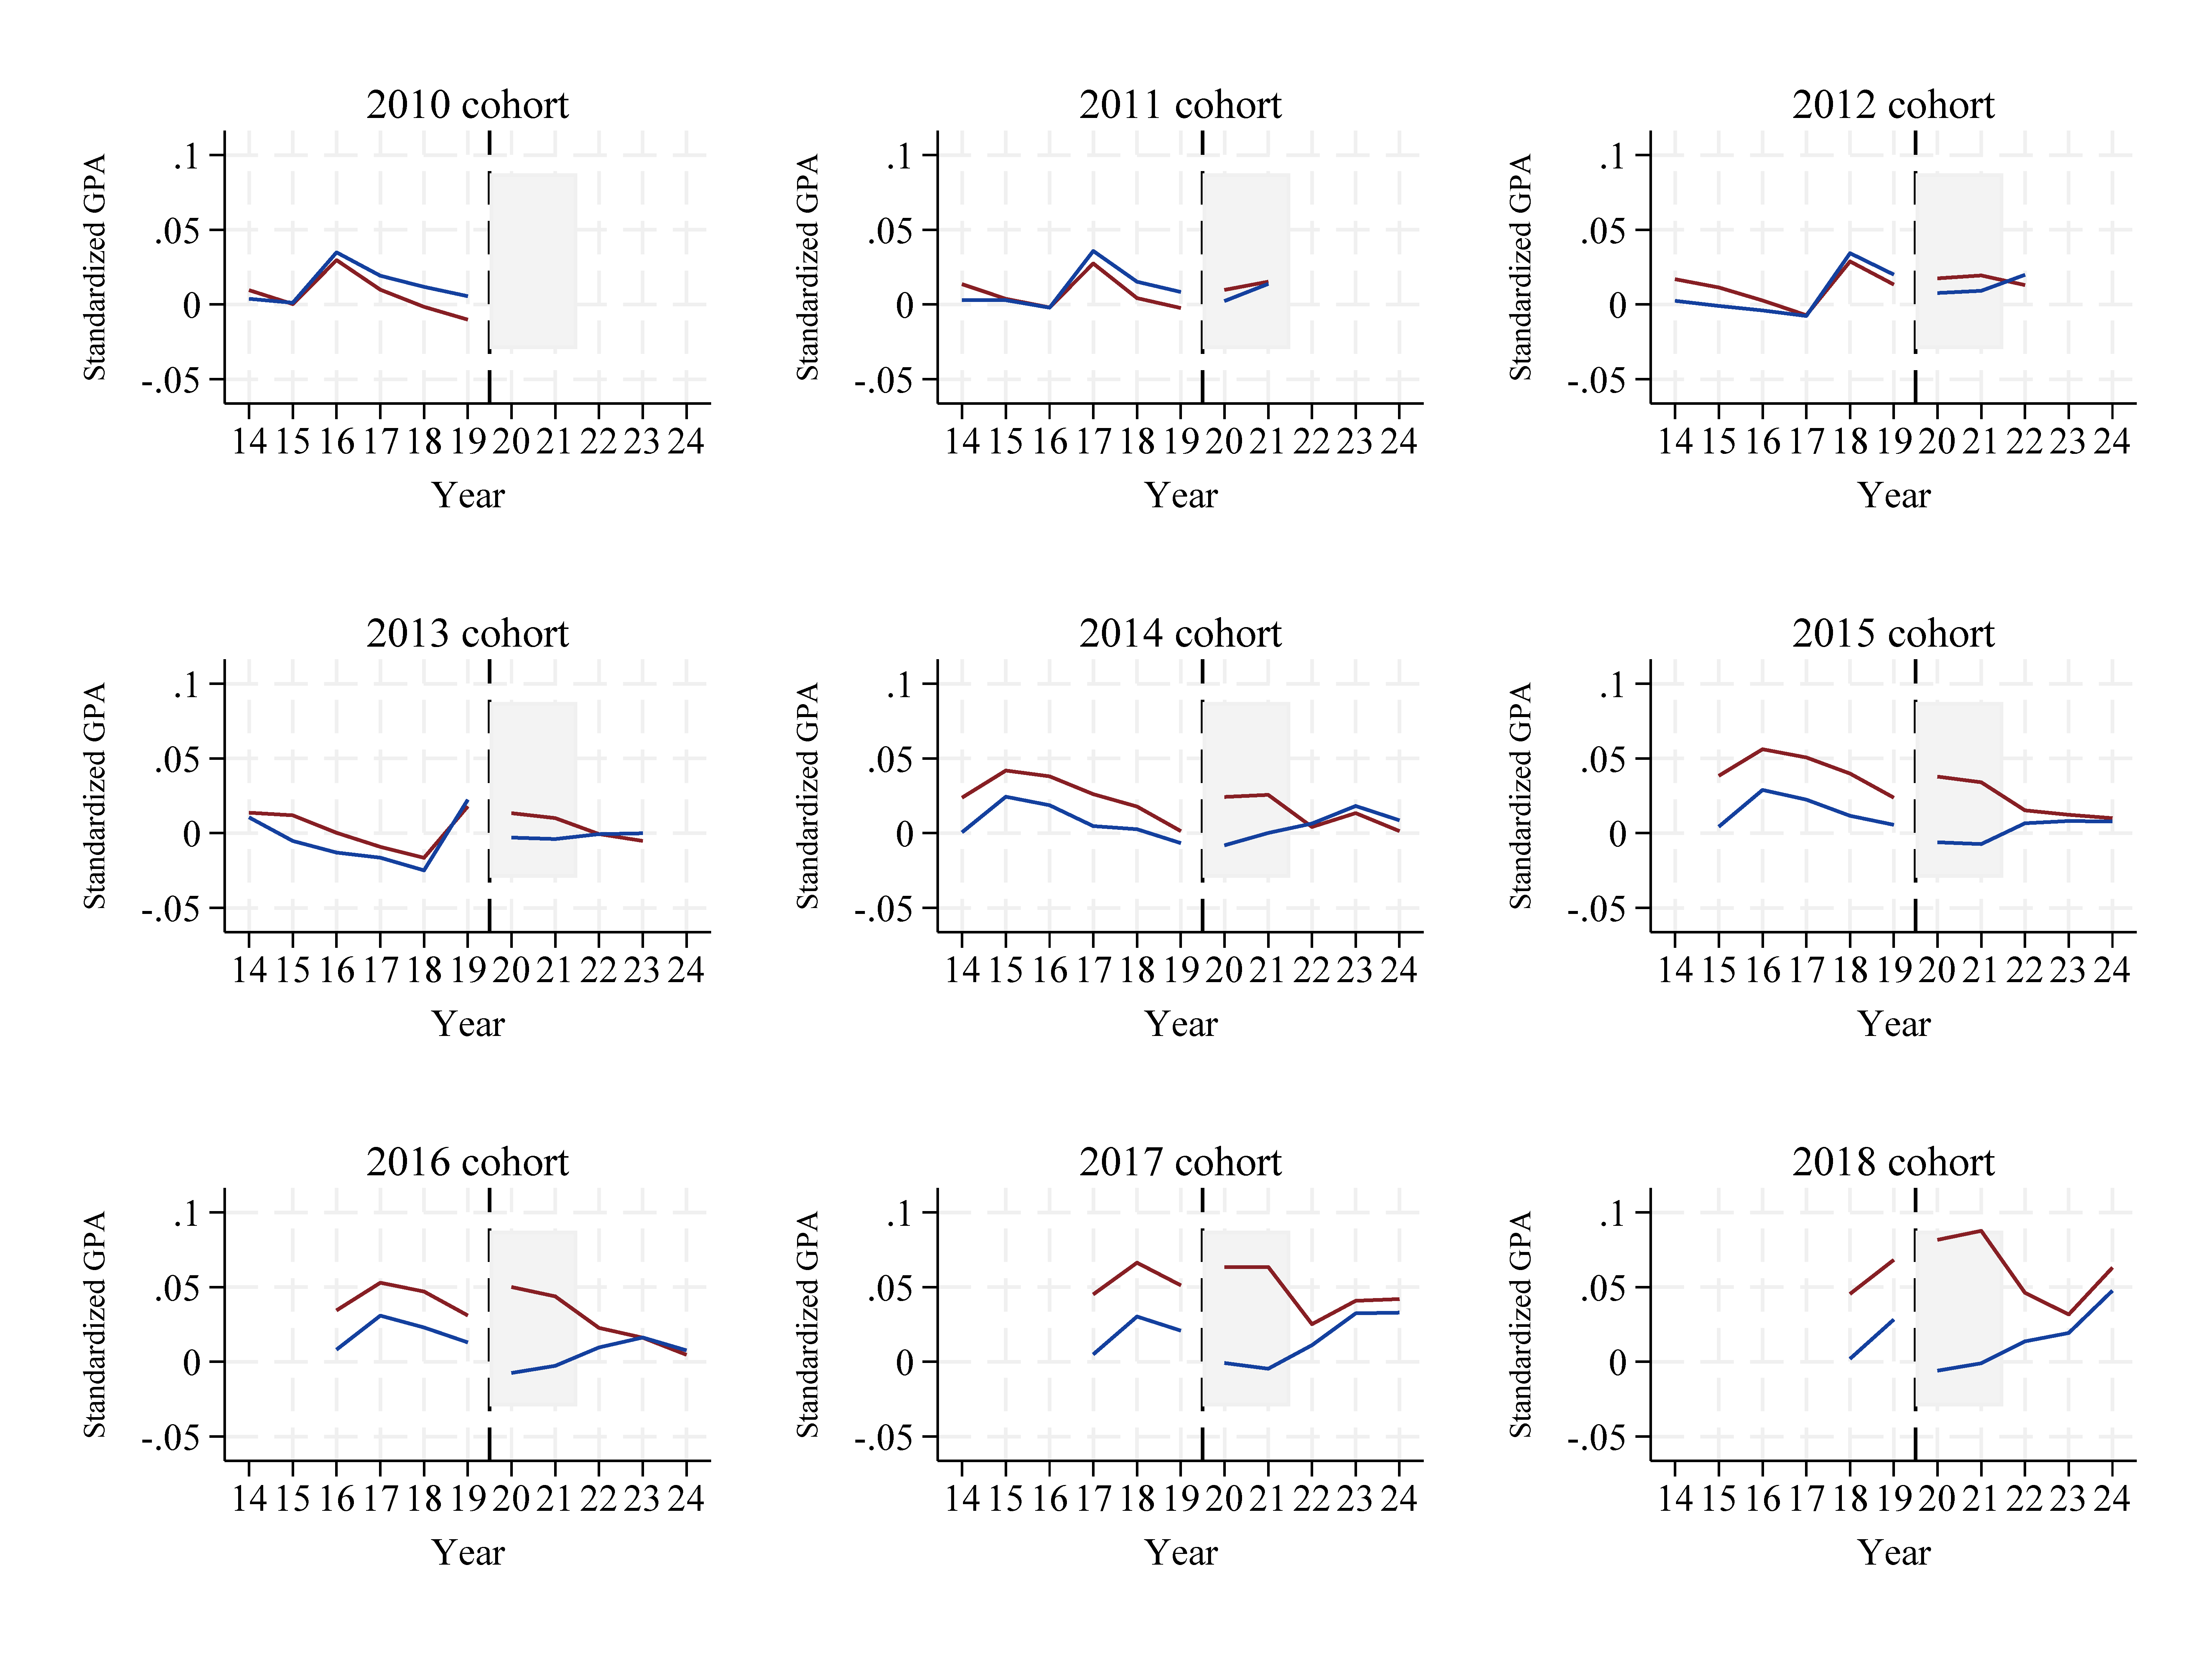
\includegraphics{./FIGURES/Descriptive/raw_cohorts_std_gpa_m.pdf}
      }
    }
\end{frame}

\begin{frame}
    \label{update_scott}
    \frametitle{Raw plots per grade - Time trend}
        {\resizebox{0.8\textwidth}{!}{
       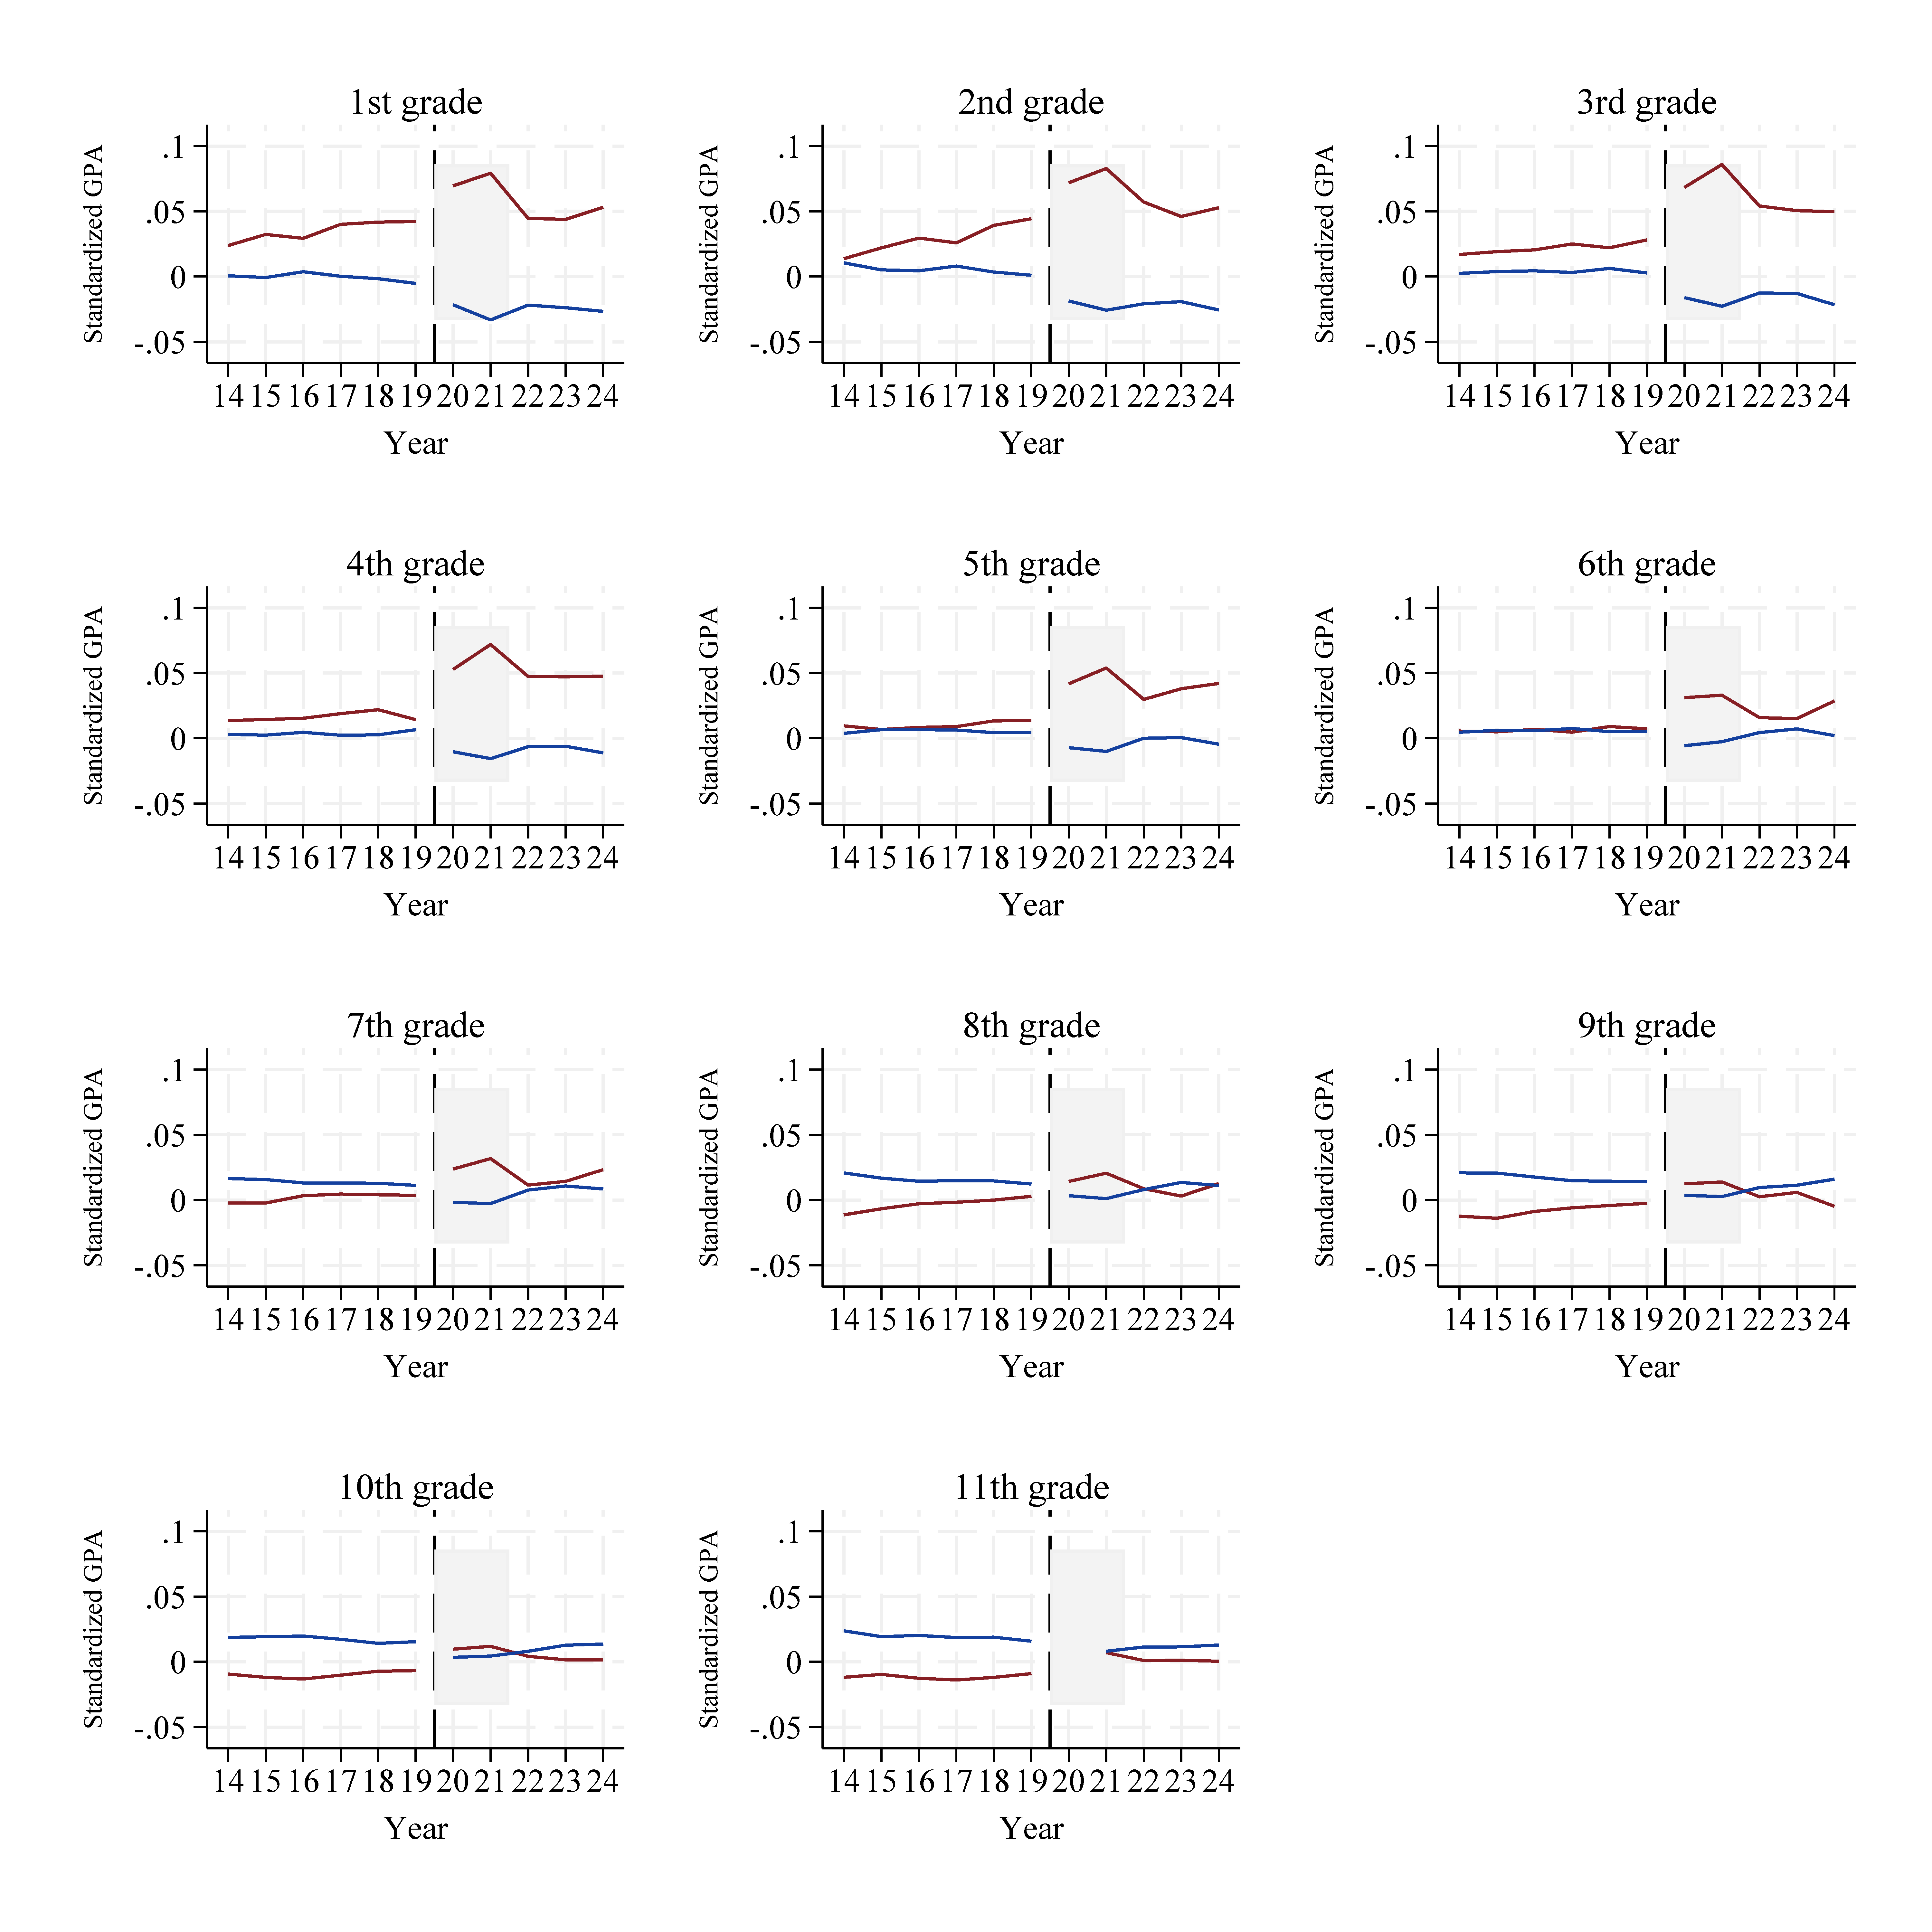
\includegraphics{./FIGURES/Descriptive/raw_grades_std_gpa_m.pdf}
      }
    }
\end{frame}

\begin{frame}
    \label{update_scott}
    \frametitle{TWFE}
 {\resizebox{0.9\textwidth}{!}{
       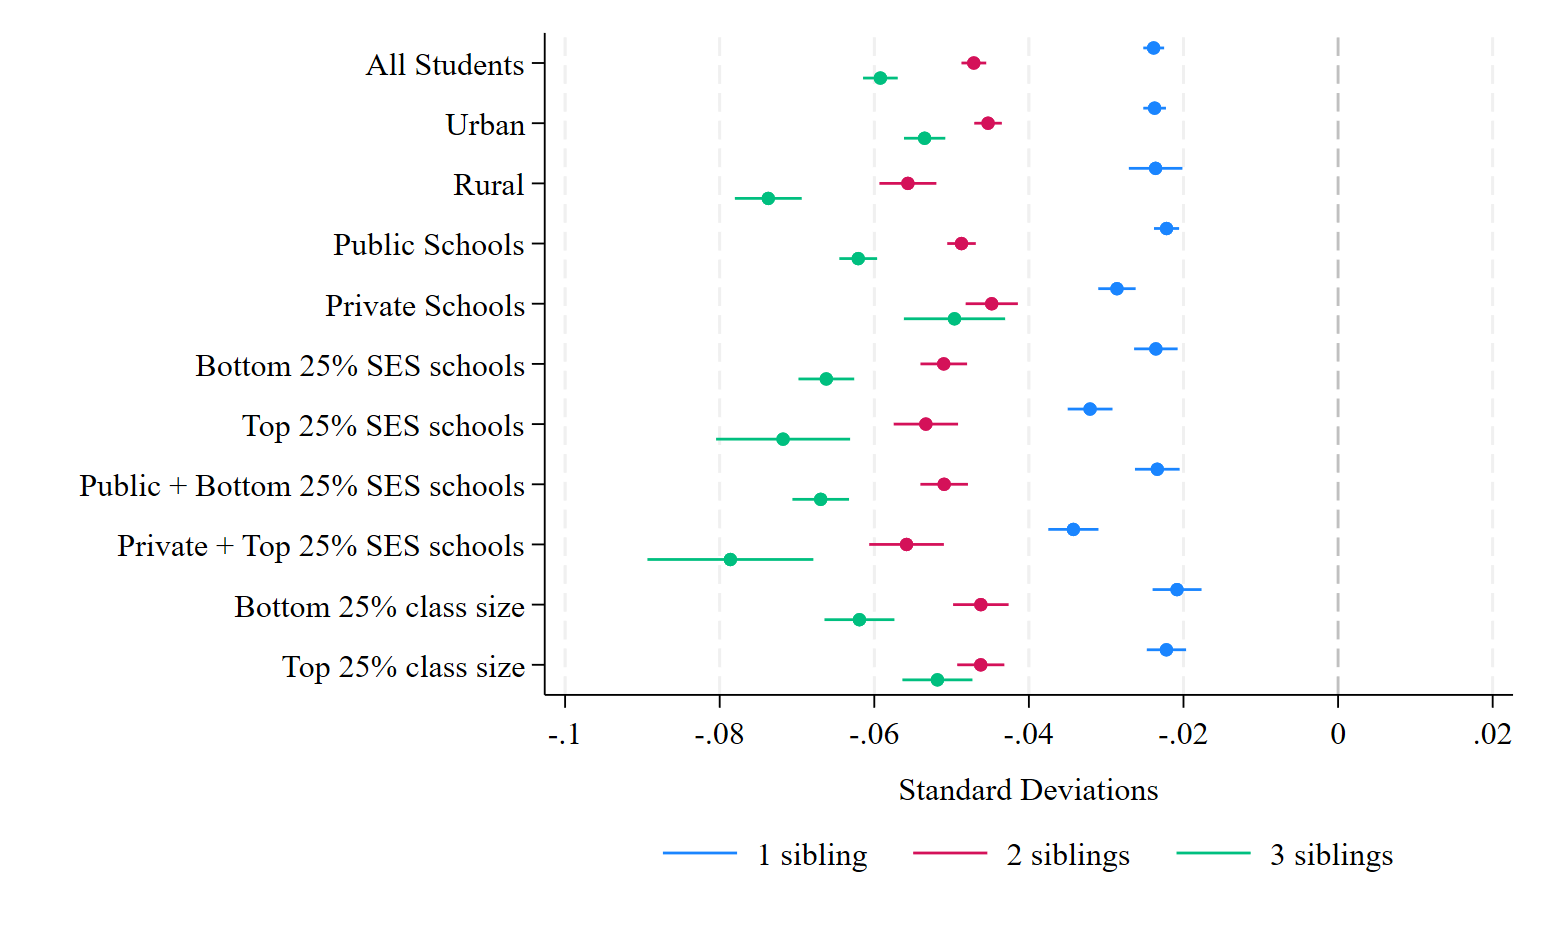
\includegraphics{./FIGURES/TWFE/covid_twfe_A_all_gpa_m_4.png}
      }
    }
\end{frame}

\begin{frame}
    \label{update_scott}
    \frametitle{TWFE}
 {\resizebox{0.9\textwidth}{!}{
       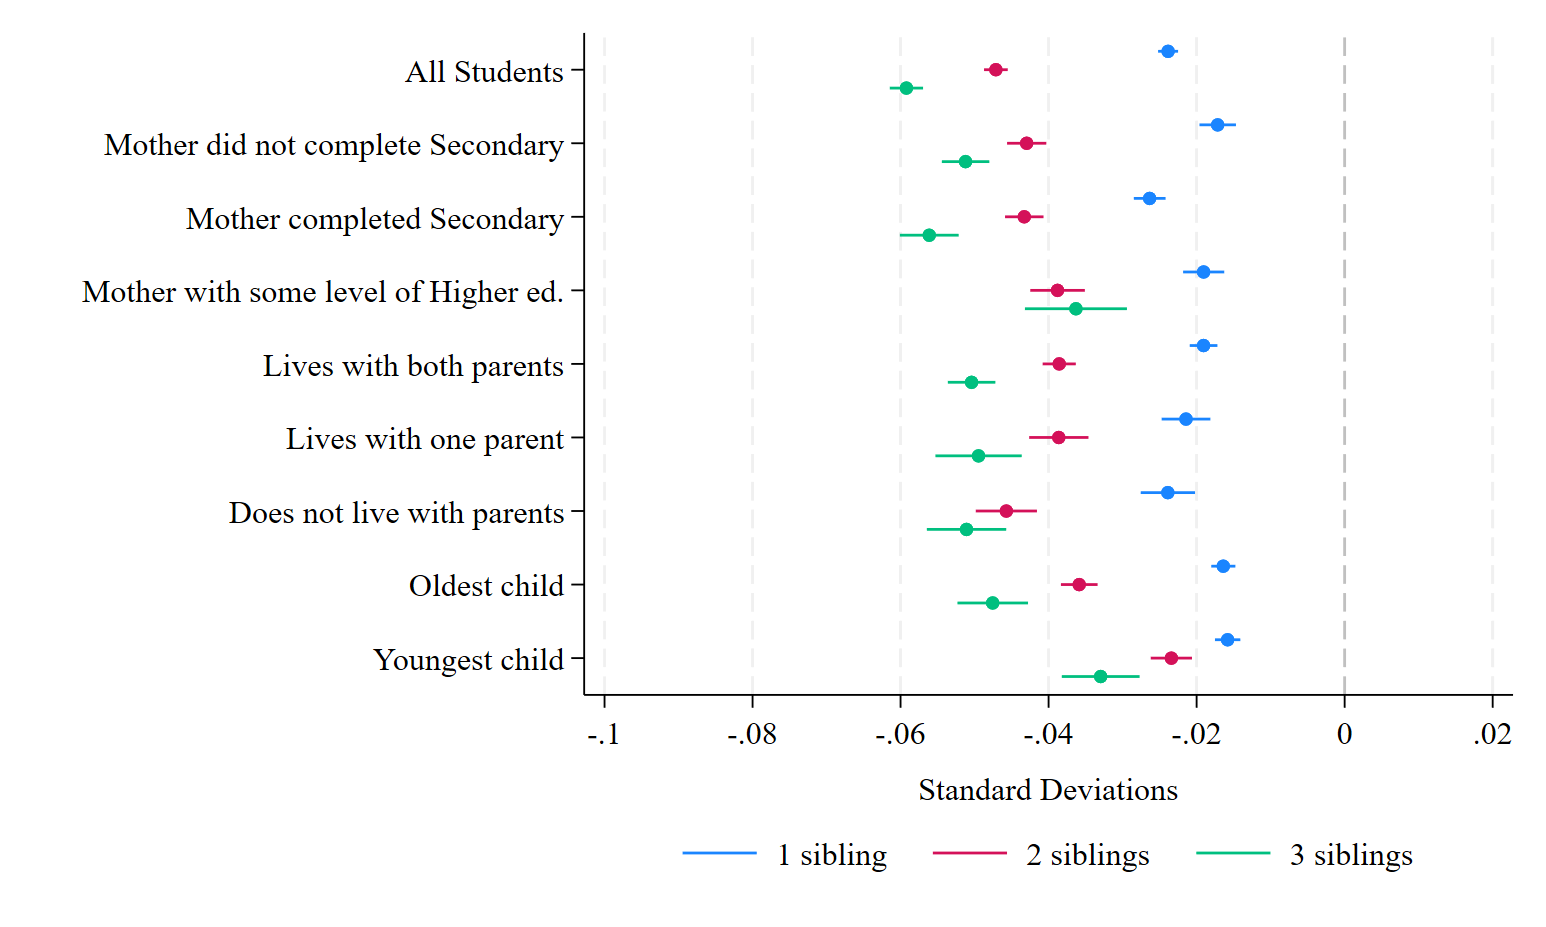
\includegraphics{./FIGURES/TWFE/covid_twfe_B_all_gpa_m_4.png}
      }
    }
\end{frame}


\begin{frame}
    \label{update_scott}
    \frametitle{School average standardized exams - 2nd grade}
        {\resizebox{0.9\textwidth}{!}{
       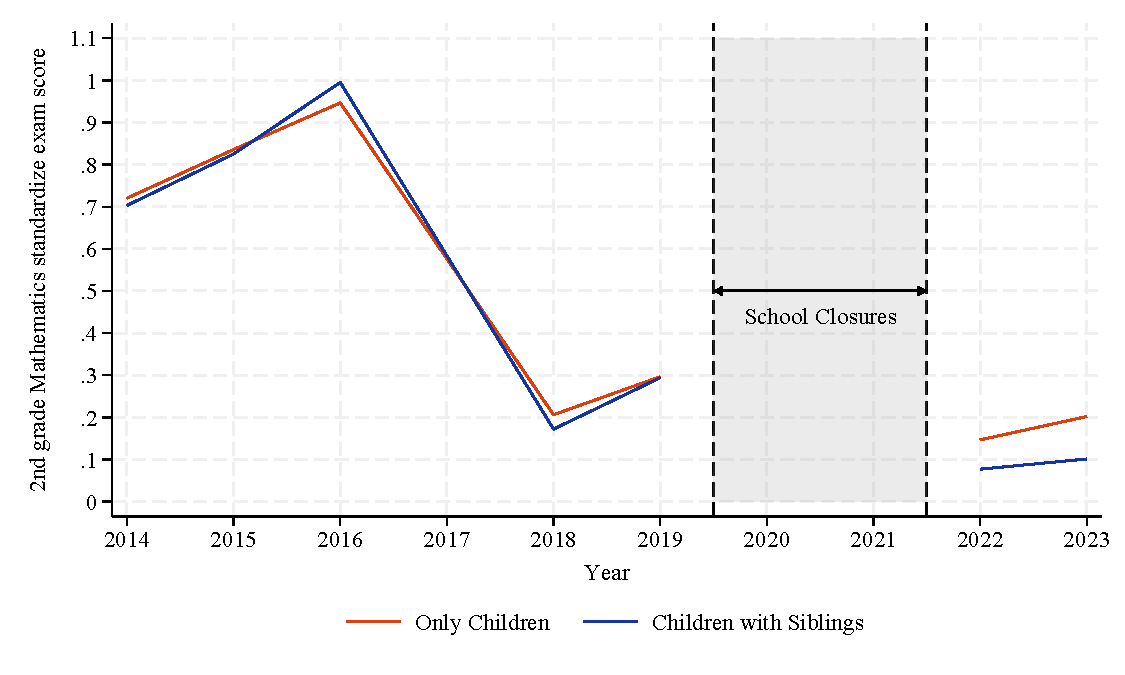
\includegraphics{./FIGURES/Descriptive/raw_ece_math_2.pdf}
      }
    }
\end{frame}

\begin{frame}
    \label{update_scott}
    \frametitle{School average standardized exams - 4th grade}
        {\resizebox{0.9\textwidth}{!}{
       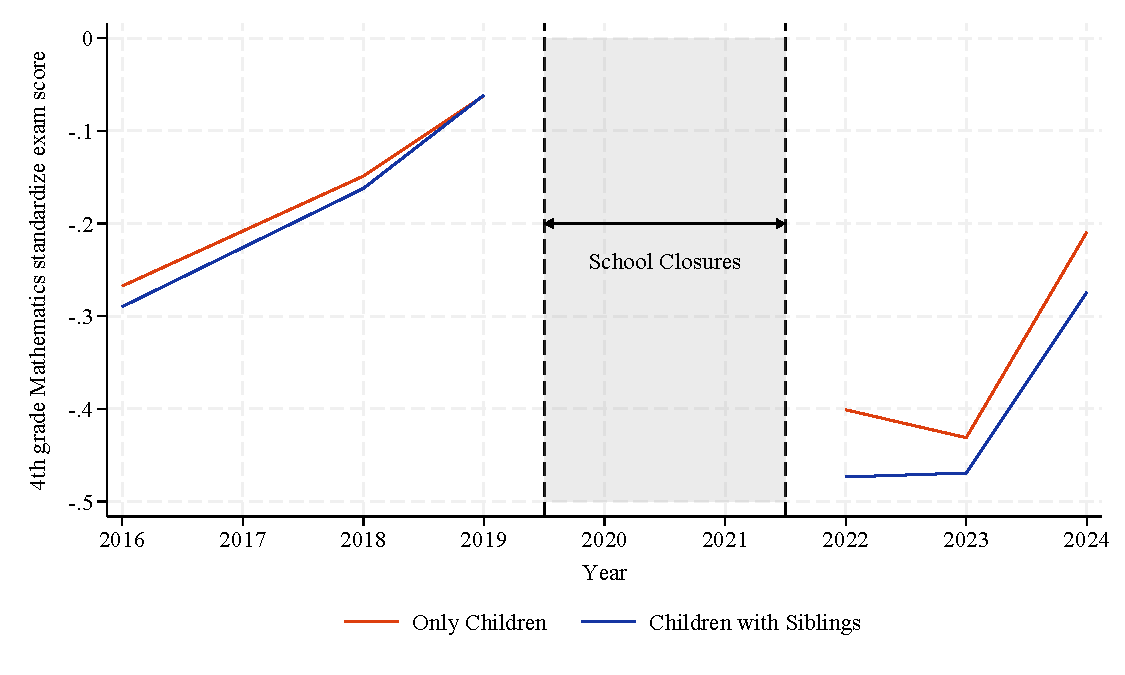
\includegraphics{./FIGURES/Descriptive/raw_ece_math_4.pdf}
      }
    }
\end{frame}

\begin{frame}
    \label{update_scott}
    \frametitle{School average standardized exams - 8th grade}
        {\resizebox{0.9\textwidth}{!}{
       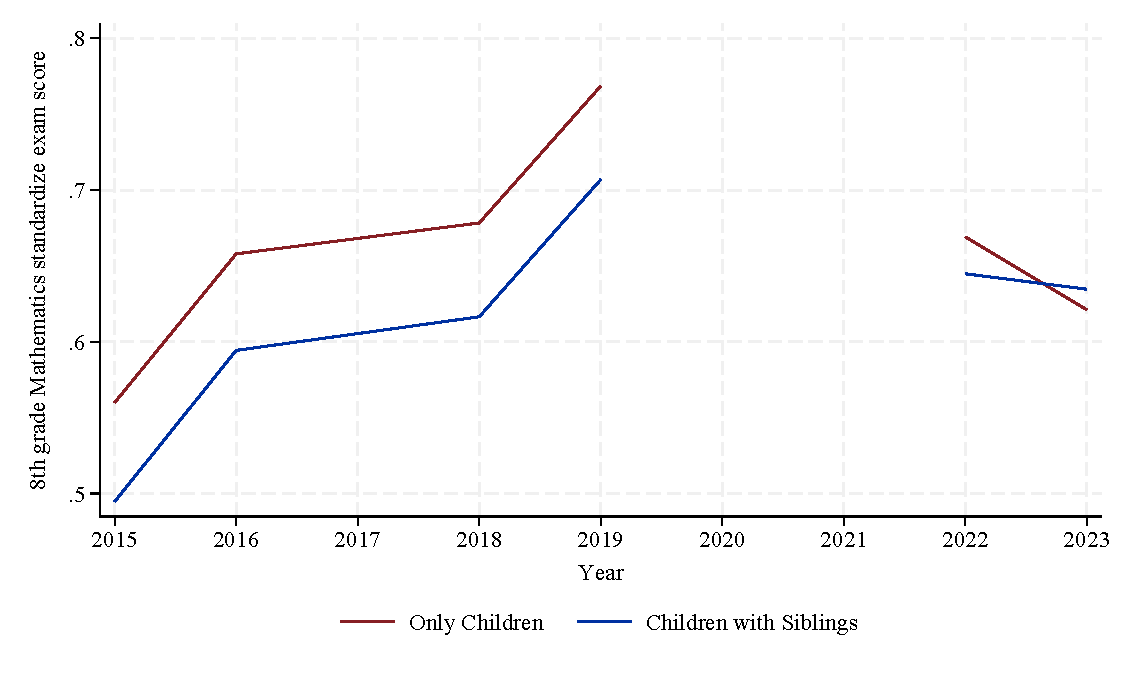
\includegraphics{./FIGURES/Descriptive/raw_ece_math_8.pdf}
      }
    }
\end{frame}


\begin{frame}
    \label{update_scott}
    \frametitle{Event Study - 2nd grade}
 {\resizebox{0.9\textwidth}{!}{
       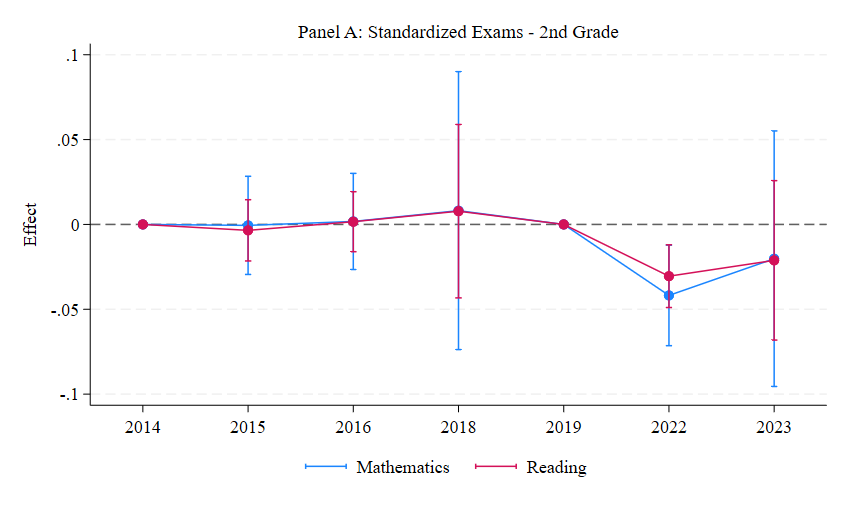
\includegraphics{./FIGURES/Event Study/ece_school_score_2p.png}
      }
    }
\end{frame}


\begin{frame}
    \label{update_scott}
    \frametitle{Event Study - 4th grade}
 {\resizebox{0.9\textwidth}{!}{
       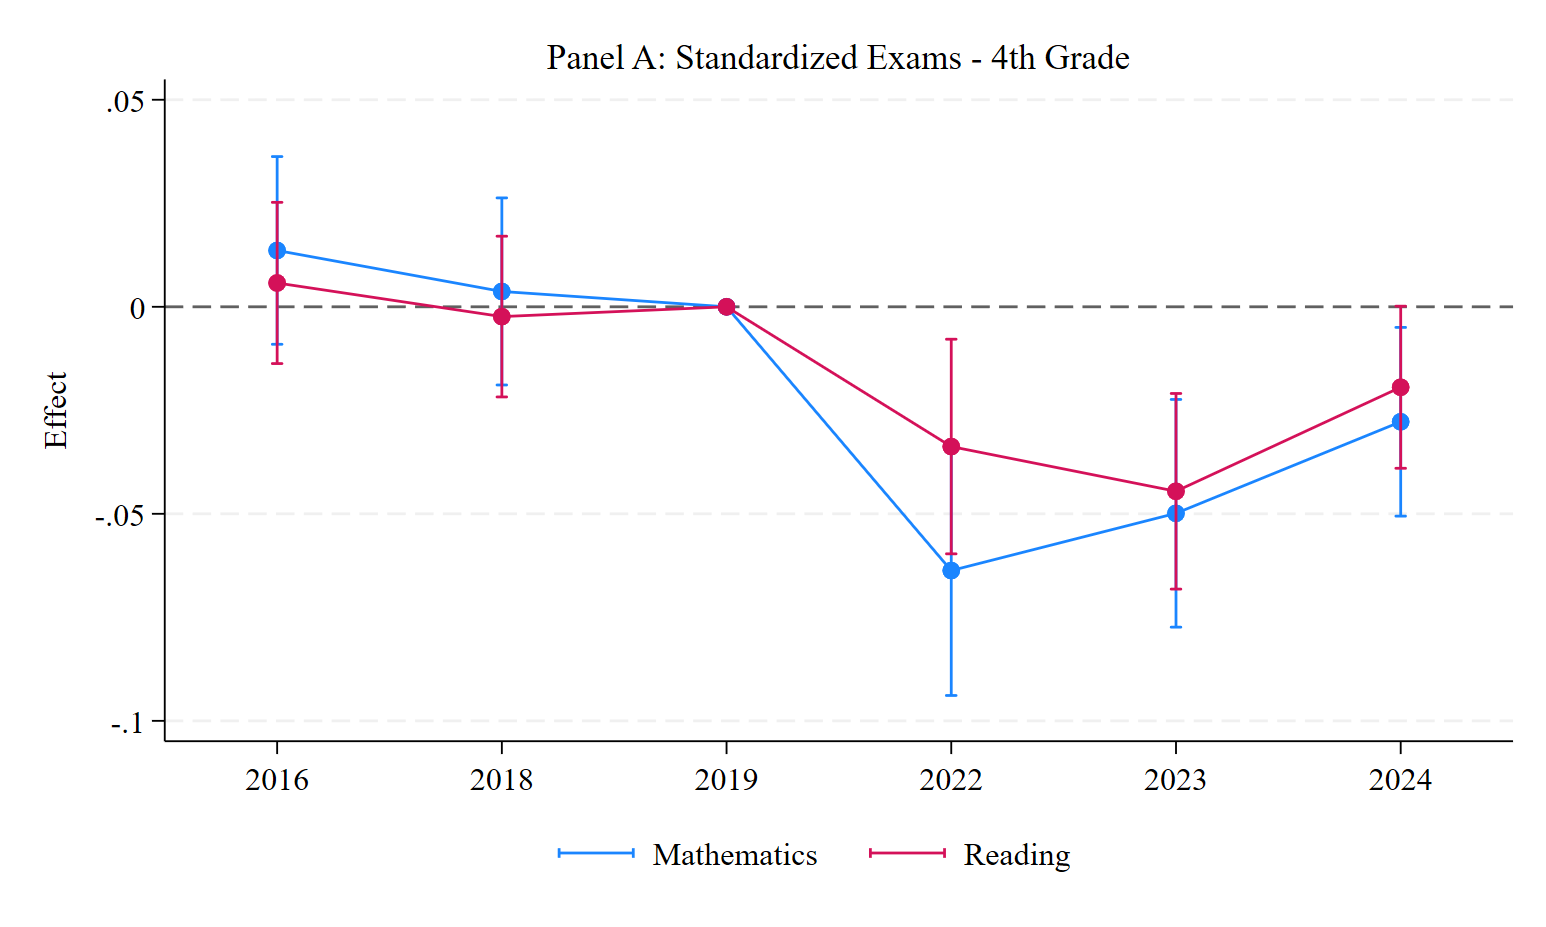
\includegraphics{./FIGURES/Event Study/ece_school_score_4p.png}
      }
    }
\end{frame}


\begin{frame}
    \label{update_scott}
    \frametitle{Event Study - 8th grade}
 {\resizebox{0.9\textwidth}{!}{
       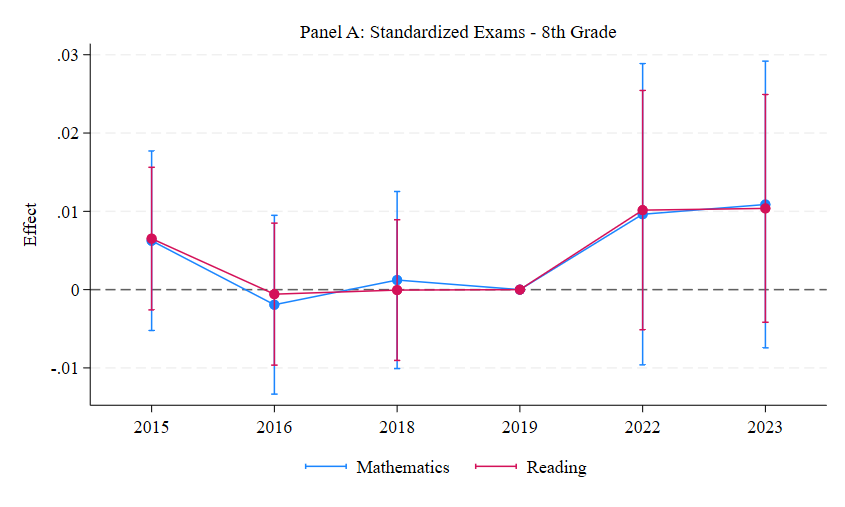
\includegraphics{./FIGURES/Event Study/ece_school_score_2s.png}
      }
    }
\end{frame}


\begin{frame}
    \label{event_cohort_m}
    \frametitle{Evidence from the Netherlands}
    \begin{itemize}
        \item Had 2 school closures during 1.5 years of Covid. $\approx$ 8 weeks of closure.
        \item Studies heterogeneity by SES, single parents, # of siblings (1-2, vs 3+). Find effects on the first, not on # of siblings.
        \item Look at learning growth across different cohorts
   
       $\Delta Y_{ijc}= \beta Post + \epsilon_{ijc}$ 
       $\Delta Y_{ijc}= \beta Post + \gamma SES + \delta Post*SES + \epsilon_{ijc}$ 
     \end{itemize}
\end{frame}


\begin{frame}
    \label{update_scott}
    \frametitle{Grade thresholds during covid}
    \begin{itemize}
        \item During covid (full academic year 2020 and 2021) all children were promoted and no subject was failed. 
        \item D grade was elimiated and grades went from 0-20 to 11-20.
        \item This could cause an spurious effect if one population was more likely below the passing grade
    \end{itemize}
\end{frame}


\begin{frame}
    \label{update_scott}
    \frametitle{Grade distributions pre-covid: Elementary}
 {\resizebox{0.9\textwidth}{!}{
       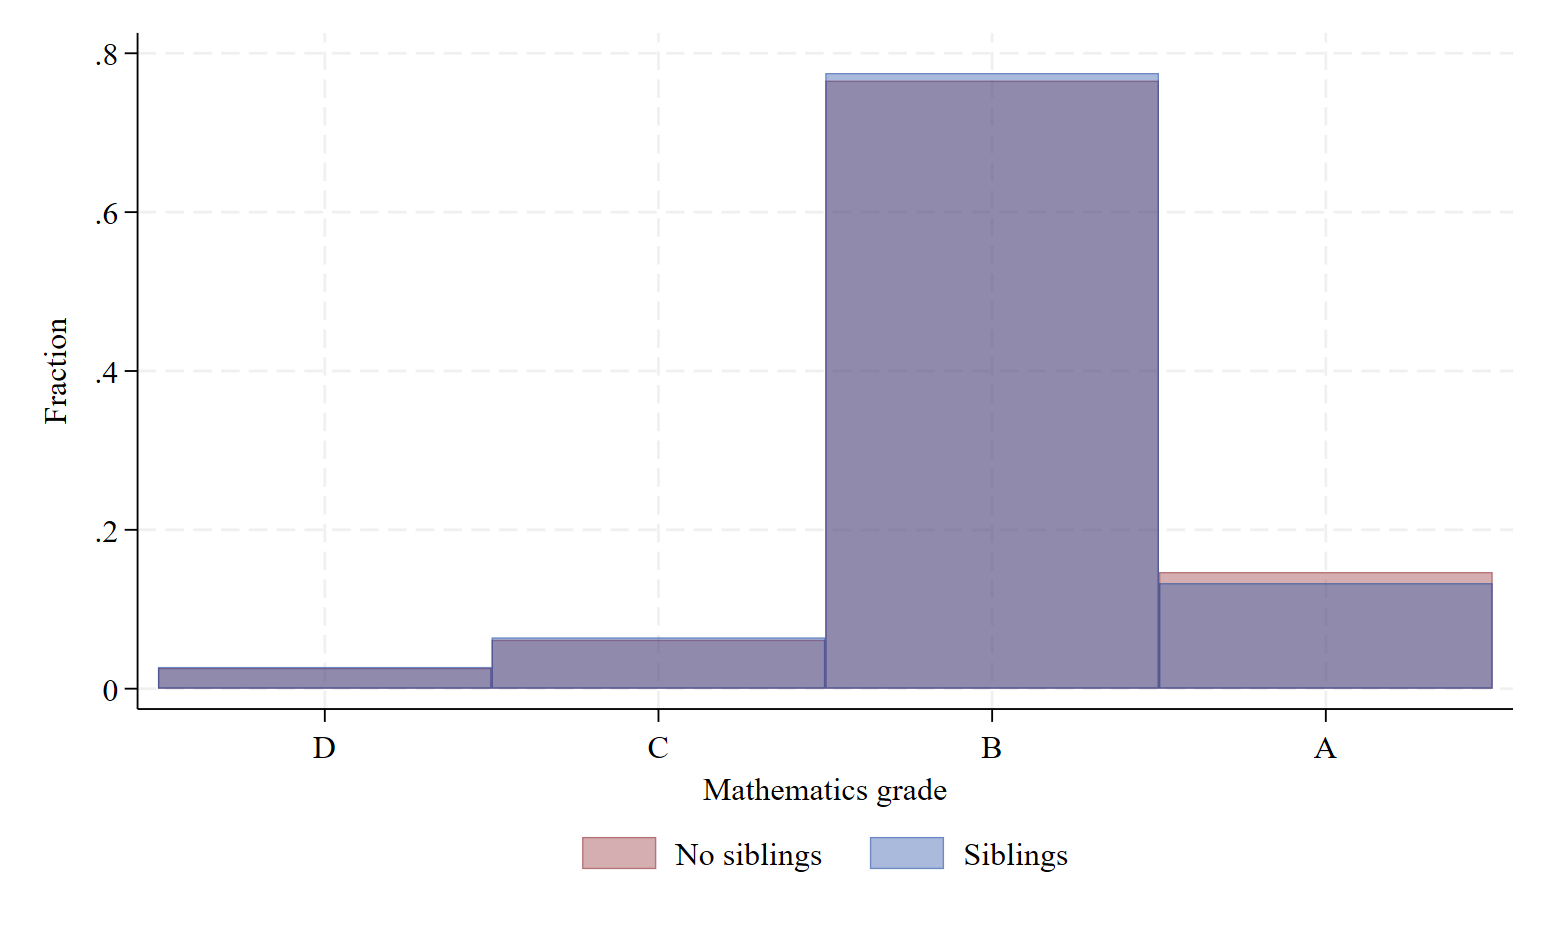
\includegraphics{./FIGURES/Descriptive/histogram_pre_elm.png}
      }
    }
\end{frame}

\begin{frame}
    \label{update_scott}
    \frametitle{Grade distributions pre-covid: Secondary}
 {\resizebox{0.9\textwidth}{!}{
       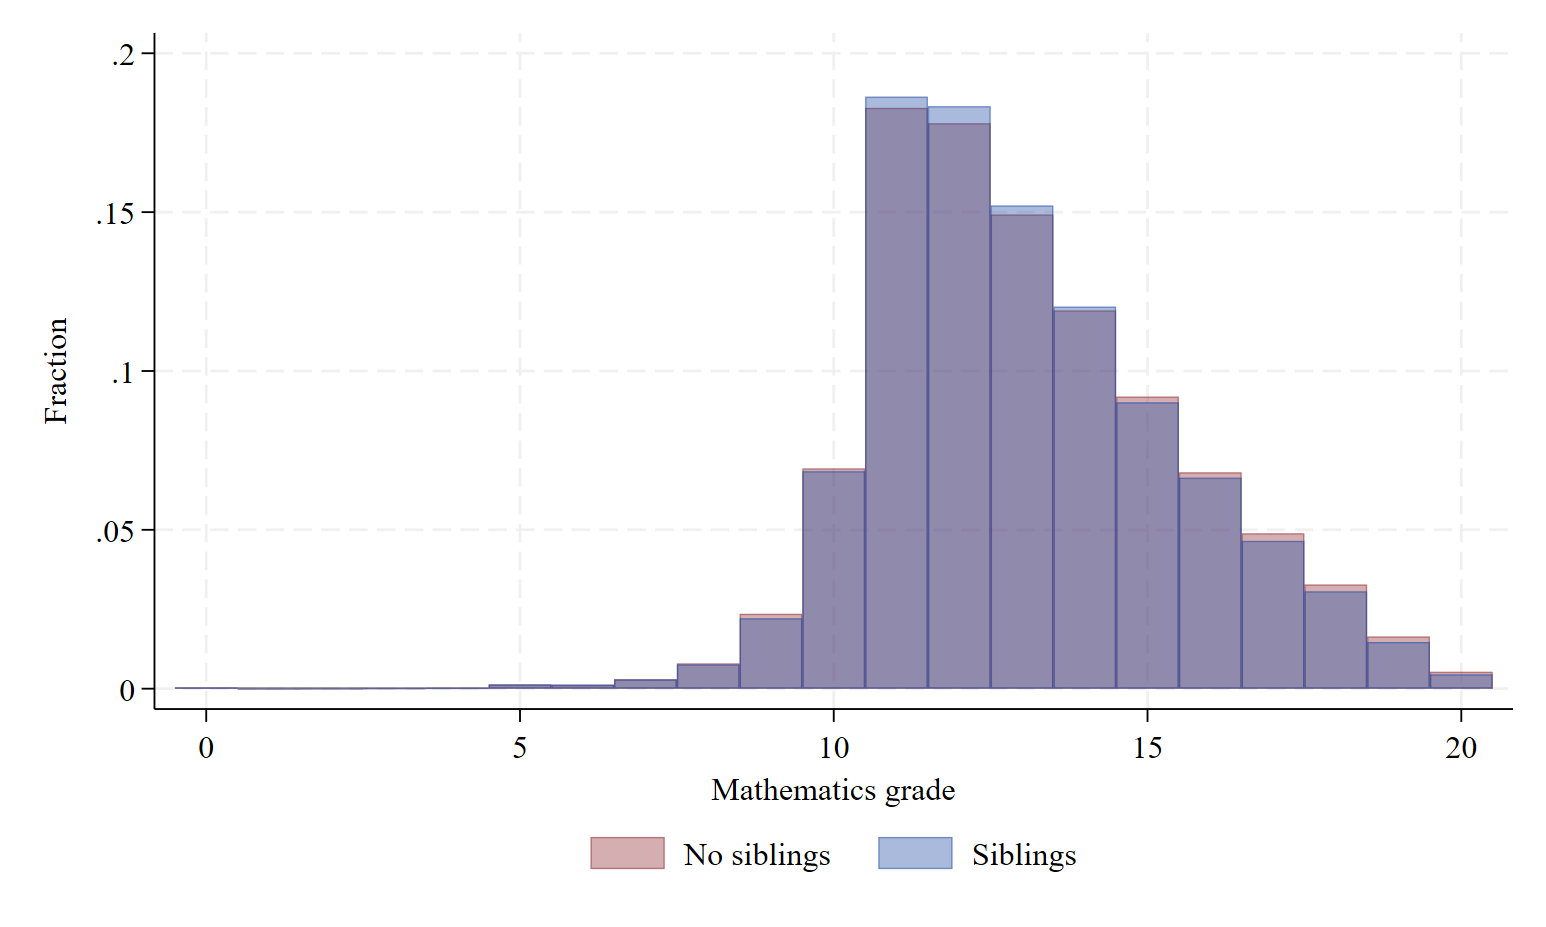
\includegraphics{./FIGURES/Descriptive/histogram_pre_9-10.png}
      }
    }
\end{frame}

\begin{frame}
    \label{update_scott}
    \frametitle{Grade distributions post-covid: Elementary}
 {\resizebox{0.9\textwidth}{!}{
       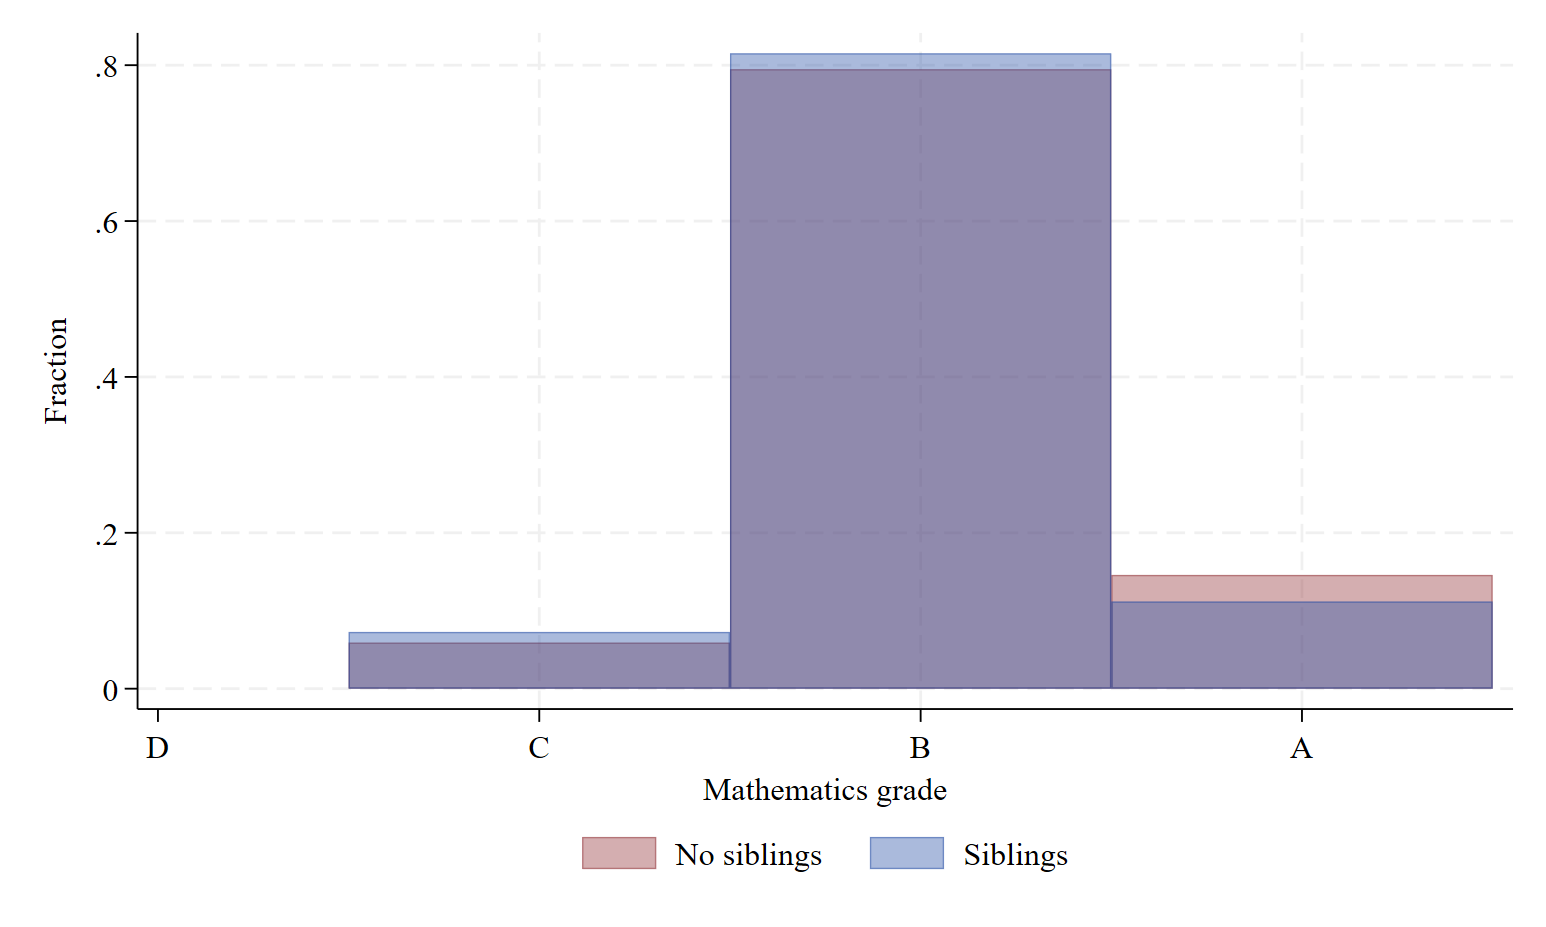
\includegraphics{./FIGURES/Descriptive/histogram_post_elm.png}
      }
    }
\end{frame}

\begin{frame}
    \label{update_scott}
    \frametitle{Grade distributions post-covid: Secondary}
 {\resizebox{0.9\textwidth}{!}{
       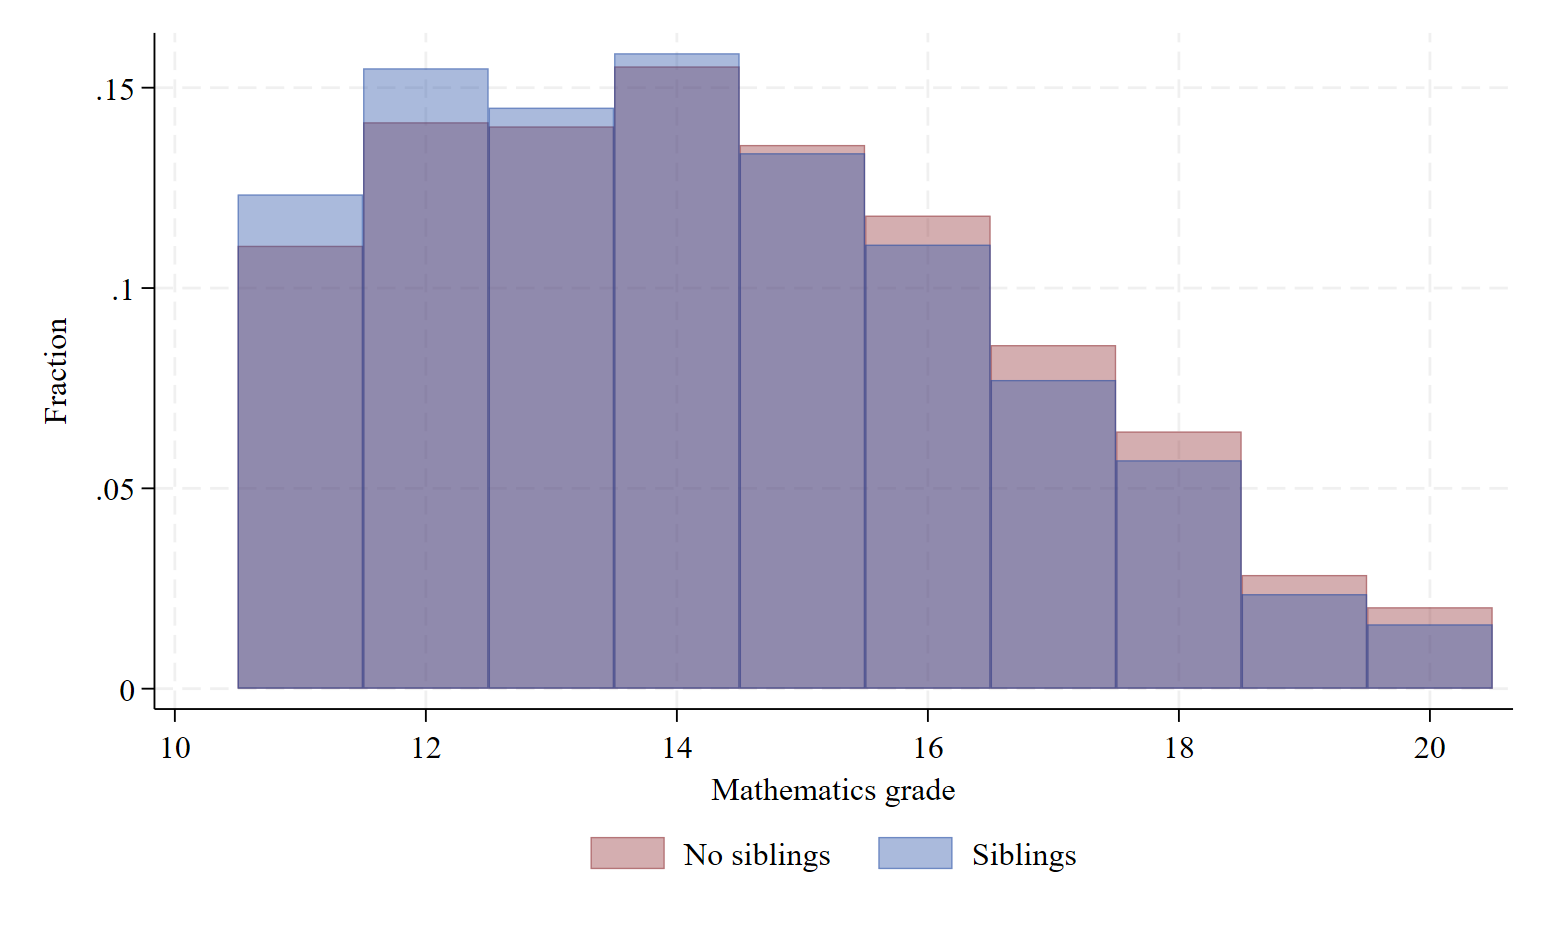
\includegraphics{./FIGURES/Descriptive/histogram_post_9-10.png}
      }
    }
\end{frame}


\section{International Evidence}


\begin{frame}
    \label{update_scott}
    \frametitle{Is this just an issue in Peru?}
    \begin{itemize}
        \item Some evidence from the Netherlands suggests it is not an issue there: No heterogeneity by number of children.
        \item I need data on:
            \begin{itemize}
                \item Educational outcomes
                \item Siblings (e.g. Do you have any?, Household size, etc)
                \item pre and post covid
            \end{itemize}
    \end{itemize}
\end{frame}



\begin{frame}
    \label{update_scott}
    \frametitle{International Achievement surveys}
    \begin{itemize}
        \item PISA
            \begin{itemize}
                \item 15 y.o.
                \item 2009-2012 and 2022 allow for sibling identification
                \item 2018 includes it for some developing countries
                \item I look at countries with observations both pre-post covid
            \end{itemize}            
    \end{itemize}
\end{frame}


\begin{frame}
    \label{update_scott}
    \frametitle{PISA: From 2009/2012 to 2022}
        {\resizebox{0.9\textwidth}{!}{
       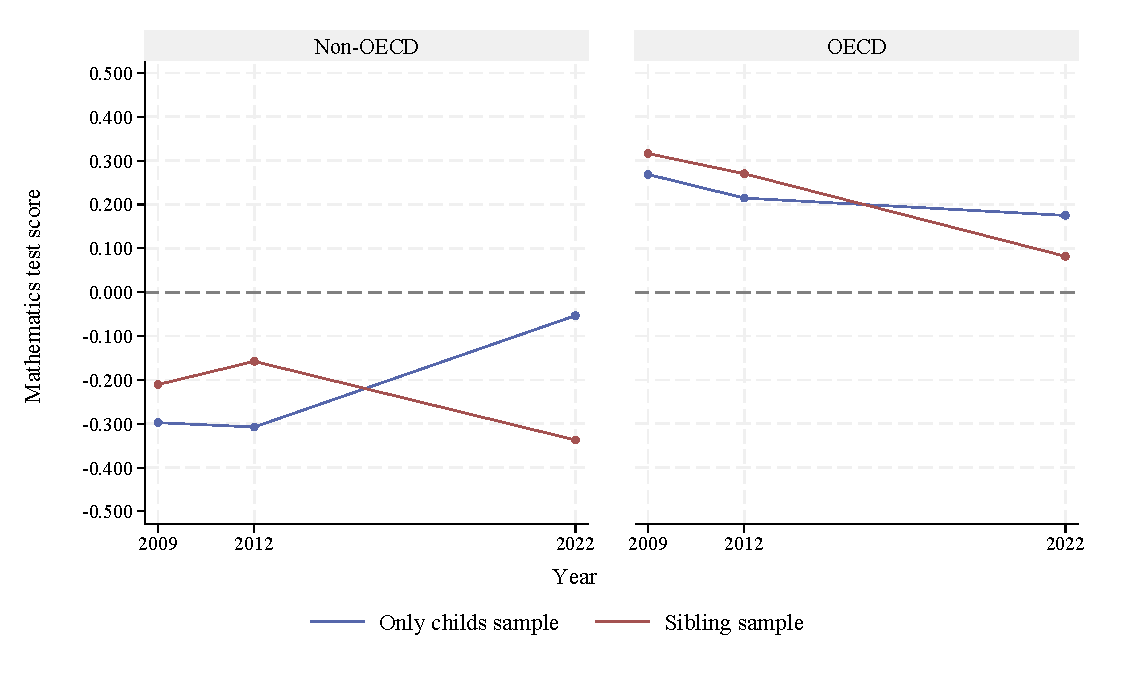
\includegraphics{./FIGURES/Descriptive/PISA_PV1MATH_2009_2022.pdf}
      }
    }
\end{frame}

\begin{frame}
    \label{update_scott}
    \frametitle{Similar Socio Economic Status}
        {\resizebox{0.9\textwidth}{!}{
       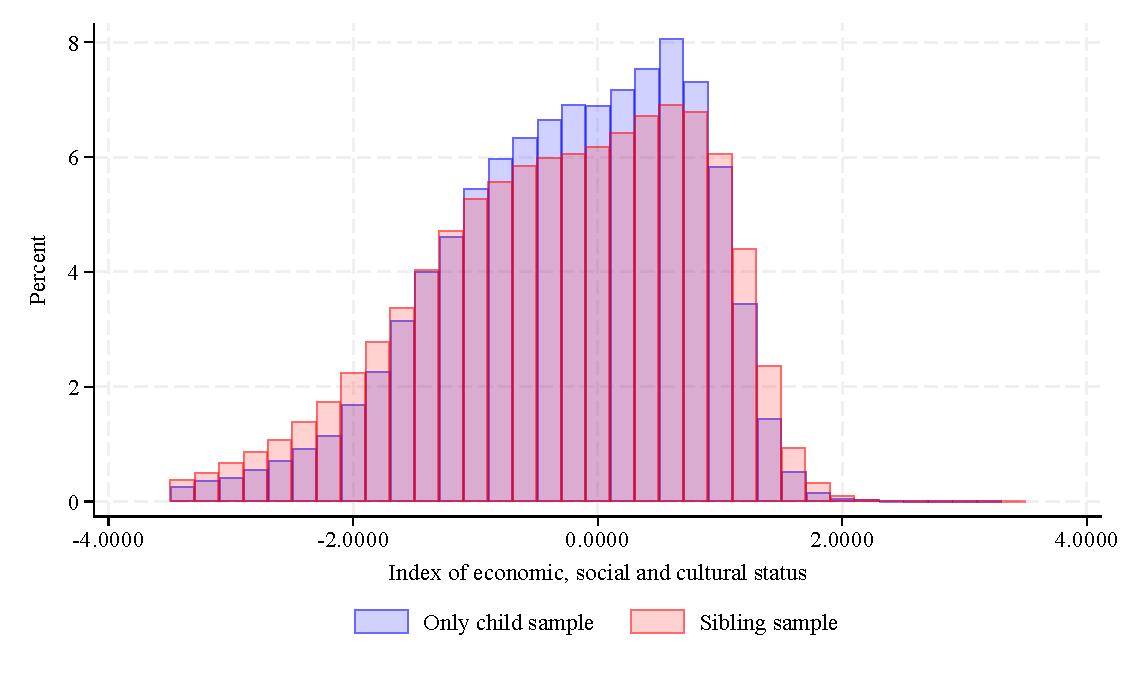
\includegraphics{./FIGURES/Descriptive/PISA_SES_2022.pdf}
      }
    }
\end{frame}


\begin{frame}
    \label{update_scott}
    \frametitle{The distribution of gaps moves down}
        {\resizebox{0.9\textwidth}{!}{
       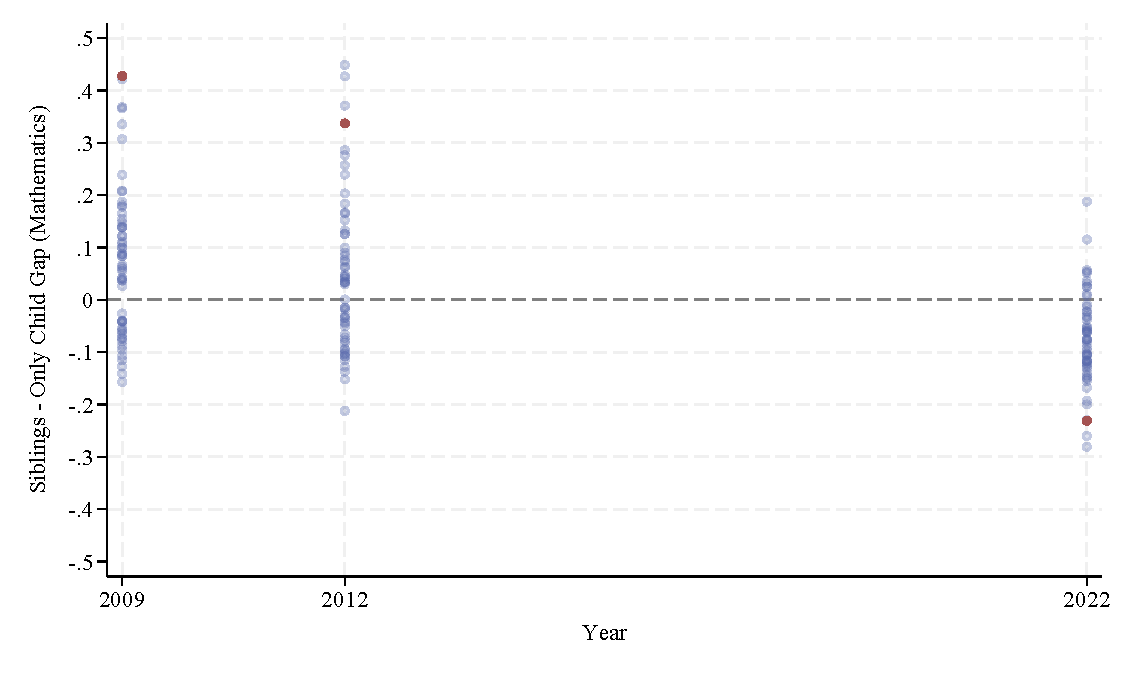
\includegraphics{./FIGURES/Descriptive/PISA_gap_PV1MATH_scatter_2009_2022.pdf}
      }
    }
\end{frame}

\begin{frame}
    \label{update_scott}
    \frametitle{PISA-D: 2018 vs 2022 (Mathematics)}
        {\resizebox{0.9\textwidth}{!}{
       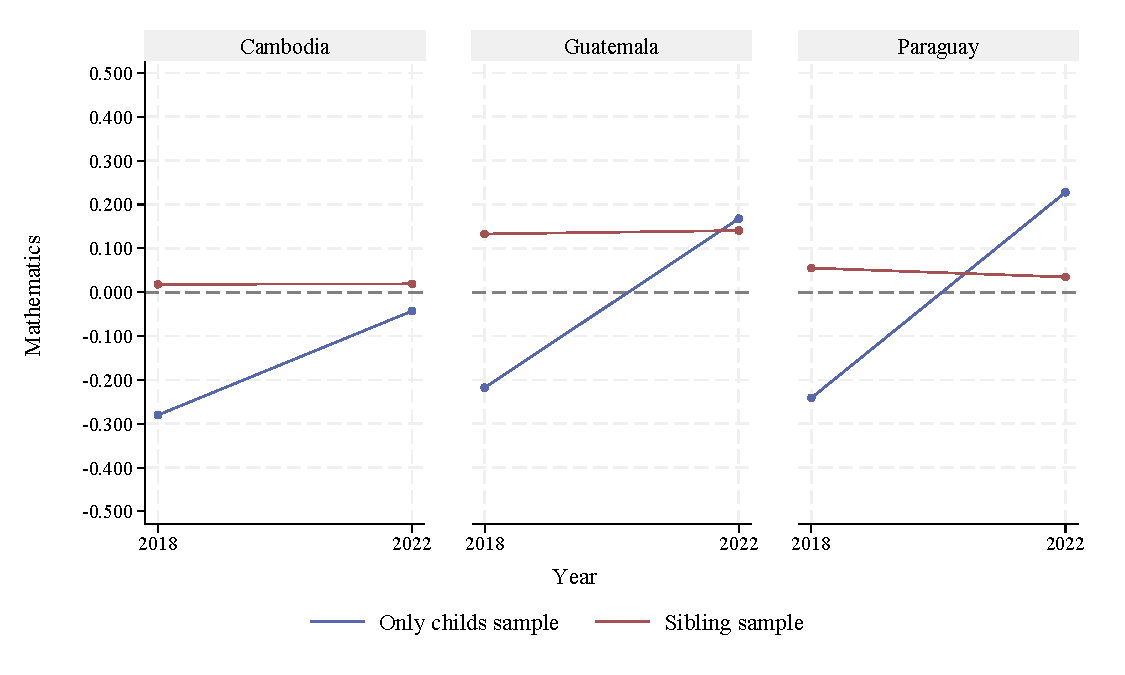
\includegraphics{./FIGURES/Descriptive/PISA_country_PV1MATH_2018_2022.pdf}
      }
    }
\end{frame}

\begin{frame}
    \label{update_scott}
    \frametitle{PISA-D: 2018 vs 2022 (Reading)}
        {\resizebox{0.9\textwidth}{!}{
       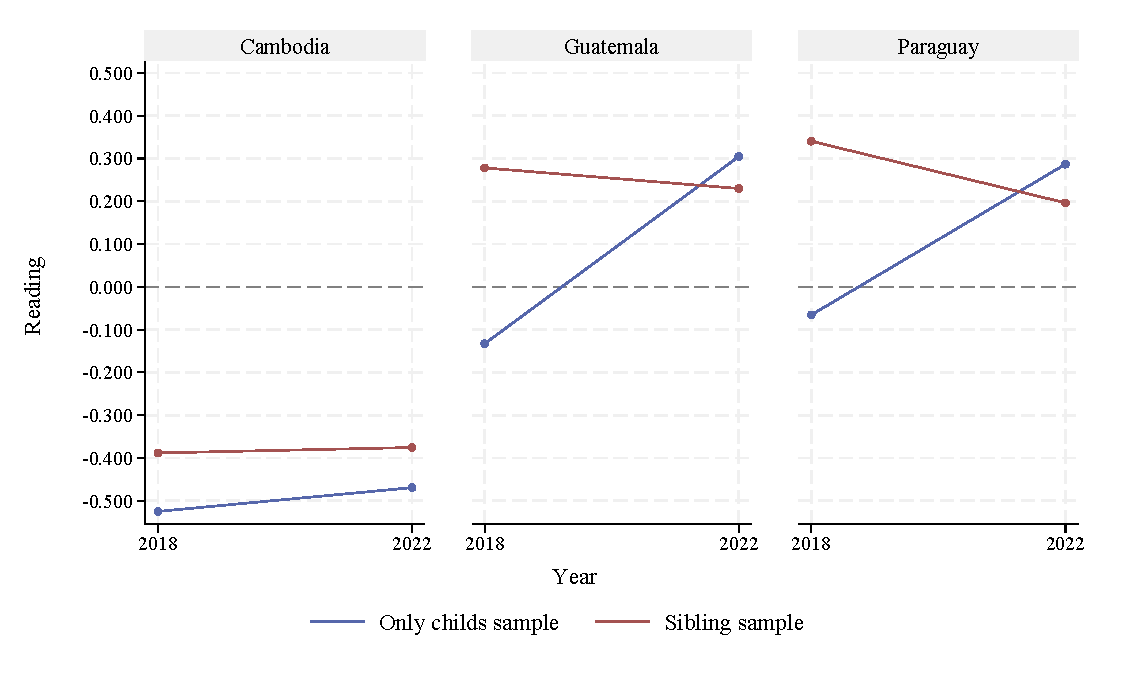
\includegraphics{./FIGURES/Descriptive/PISA_country_PV1READ_2018_2022.pdf}
      }
    }
\end{frame}


\begin{frame}
    \label{update_scott}
    \frametitle{Motivation}
    \begin{enumerate}
        \item Persistent learning losses from Covid-19
        \item \textbf{Universal PreK:} \\
        $\uparrow$ labor and earnings. Benefits $>>>$ Costs. \\
        \small \textcolor{grey}{Jackson, Turner, Bastian (2025), Humphries et al (2025)}
    \end{enumerate}
\end{frame}

\begin{frame}
    \label{update_scott}
    \frametitle{Contribution to literature}
    \begin{enumerate}
        \item \textbf{Covid Learning Loss} \\
        \item \textbf{Parental Investment} \\
        \item \textbf{Quanity-Quality} \\

    \end{enumerate}
\end{frame}






\begin{comment}
\begin{frame}
    \label{update_scott}
    \frametitle{List of Countries}
       \begin{itemize}
           
       \end{itemize}
    
\end{frame}
\end{comment}

\end{document}